%!TEX root = ../Thesis.tex

\chapter{Sub-Aperture Correlation Imaging}\label{chap:SASACI}

\graphicspath{{SASACI/Images/}{SASACI/Images/Apodizations/}{SASACI/Images/ApertureSize/}}

\section{Background}
The objective of developing this novel advanced signal processing method is to combine time and spatial domain based algorithms to increase the SNR of ultrasound images while maintaining an acceptable resolution for defect detection and characterisation during the inspection of materials with high levels of structural noise. 

TFM works very well on homogeneous, isotropic materials and is often referred to as the `gold standard' in ultrasonic NDE\cite{fan_comparison_2014}; however the results produced from TFM in highly scattering materials can suffer from degradation\cite{lane_inspection_2010}. The large grain boundaries within these materials cause incident ultrasonic energy to scatter which gives rise to speckle noise and lowers the SNR of the resultant image.

Phase Coherence Imaging proposes using the Phase Coherence Factor (PCF) to determine whether or not a signal at a given point is predominantly noise or from a legitimate reflector\cite{camacho_phase_2009}. PCF calculates the instantaneous phase of each A-scan over the whole FMC dataset before applying delays. Unlike delay-and-sum, PCF calculates the standard deviations of the phases for a focal point. The lower the standard deviation, the less likely it is that the signal is speckle noise. The PCF can be used to weight delay-and-sum images, or even TFM. Experiments in the medical field have shown the PCF is also able to reduce main lobe width as well as sidelobe intensity. Reduction of the main lobe width is desirable as it can lead to a potential increase in resolution. In NDE, PCF has been shown to lower sidelobe levels and improve resolution, but the improvement is not significant for some materials of interest, high nickel alloys for example\cite{camacho_phase_2011}. PCF has limitations when applied to data from materials in which multipath propagation is an issue. Multipath propagation causes phase aberration with resultant problems in generating an accurate phase coherence factor. 

The Generalised Coherence Factor (GCF), proposed by Li and Li\cite{li_adaptive_2003} uses a similar principle to generate a weighting function based on the statistical likelihood that a signal is predominantly noise. For each point to be analysed, GCF performs the requisite delays before summing for a range of time samples around the desired sample. An FFT is performed and the frequency spectrum of the signal is analysed. The GCF is defined by the ratio of low frequency energy in the signal to total energy. Furthermore, GCF as a weighting function has been shown to effectively reduce speckle noise.

Dual Apodisation with Cross-Correlation (DAX) has shown promise in reducing speckle noise in medical ultrasound. Introduced by Seo and Yen \cite{seo_sidelobe_2008}, DAX uses two apodisation functions alongside basic Delay and Sum beamforming to create opposing signals with out of phase grating lobes, which are then cross-correlated. Seo proposed four different apodisation methods in his paper: Alternating, Common Midpoint, Random and Hamming Windowed. The alternating method created two opposing apertures consisting of the odd and even numbered apertures respectively. The random method selects a random set of $\frac{n}{2}$ elements from the $n$ element array. The common midpoint method uses the central array elements in both apertures and assigns the elements from each end of the array their respective signals. The windowing method applies a window across all of the array elements for one set of signals and uses a rectangular window across the other set. A high correlation coefficient at a certain point means that both of the signals are similar and that the signal at the point is likely to be from a reflector. Conversely, a low correlation coefficient will mean that the signals are unrelated and are likely to be either contributions from the sidelobe, or speckle noise. DAX has shown promise in medical ultrasound imaging and is the inspiration for the technique presented in this chapter.

The motivation behind developing a new method is straightforward. The aforementioned techniques are designed to be applied using an approach based on the focused B-scan imaging methodology. The Full Matrix Capture records a larger volume of data that can be used in post-processing and TFM-based imaging techniques can be applied that will offer a higher resolution and SNR while reducing the point spread when comparing to focused B-scan inspired techniques\cite{holmes_post-processing_2005}.

\section{Theory}
\subsection{Overview}
This chapter presents a novel imaging algorithm designed to reduce the contributions from sidelobes when inspecting ultrasonically noisy materials. It has been called Sub-Aperture Spatially Averaged Correlation Imaging (SASACI) and combines the focusing qualities of TFM with the sidelobe reducing properties of DAX\cite{seo_sidelobe_2008}.

Any ultrasound signal received from a pulse-echo measurement can be thought of as the sum two discrete signals, reflections from the main lobe and reflections from sidelobes. The energy reflected from sidelobes is considered to be noise which will reduce the image contrast and possibly add speckle to an image. SASACI minimises the contributions from the reflection of sidelobes. To do this, contributions from the main lobe must be differentiated from contributions from reflections in the clutter region. As seen from the flowchart in Figure~\ref{fig:sac_flowchart}, SASACI operates on an FMC data set and is strongly linked to the Total Focusing Method.

\begin{figure}[htp]
\centering
		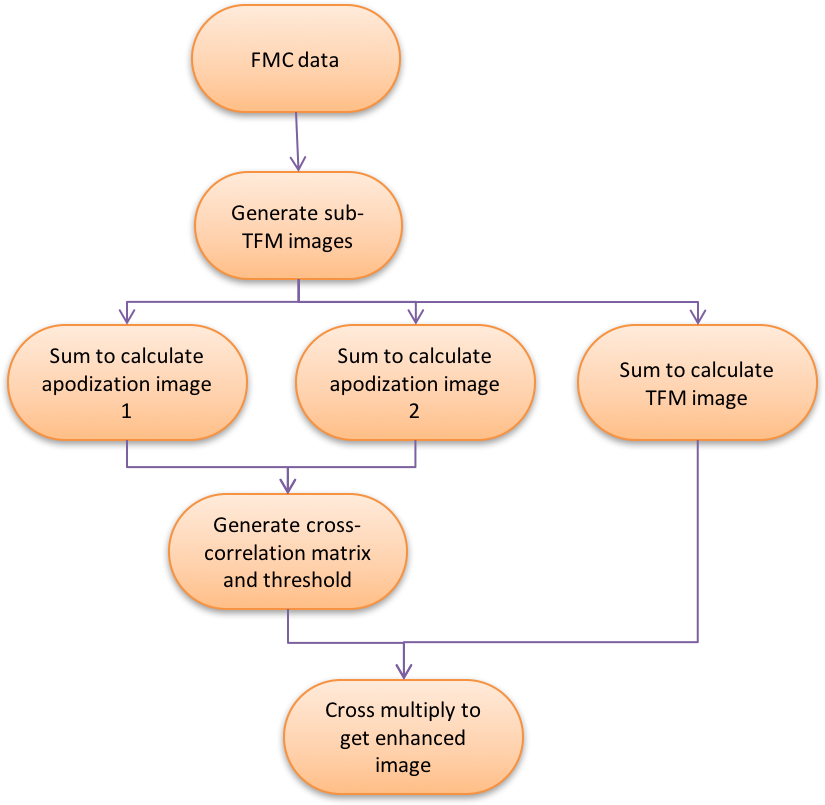
\includegraphics[width=\textwidth]{flowchart.png}
		\caption{SASACI Methodology}
		\label{fig:sac_flowchart}
\end{figure}

\subsection{SASACI}\label{sec:sasaci}
SASACI is based on the same principle as TFM, introduced in Section \ref{sec:TFM}, but aims to extract additional information from the same FMC data. SASACI creates an image for every transmitting element for which data has been acquired. The set of images is generated using Equation~\ref{eq:SubTFM}, which uses the same general concept as the Total Focusing Method. The only difference between Equations \ref{eq:TFM} and \ref{eq:SubTFM} is that the data from the transmitting elements will contribute to individual images, as demonstrated by the variable $SubTFM_{tx}$ which is a matrix of images. These images will be referred to as Sub-TFM images and the sum of all these images will be equal to a standard TFM image. Figures \ref{fig:sactfm1} and \ref{fig:sactfm2} show a graphical representation of this concept. In Figure \ref{fig:sactfm1}, a TFM image is generated by summing the contributions for each transmit-receive pair of elements. In Figure \ref{fig:sactfm2}, a separate image is generated for each element, using every contribution from individual transmitting elements for each separate image.

 \begin{equation} \label{eq:SubTFM}
SubTFM_{tx}(y,z) = | \sum h_{tx,rx} (\frac{\sqrt{(y_{tx} - y)^2 + z^2} + \sqrt{(y_{rx} - y)^2 + z^2}}{v_L}) |
 \end{equation}

\begin{figure}[htb]
\centering
		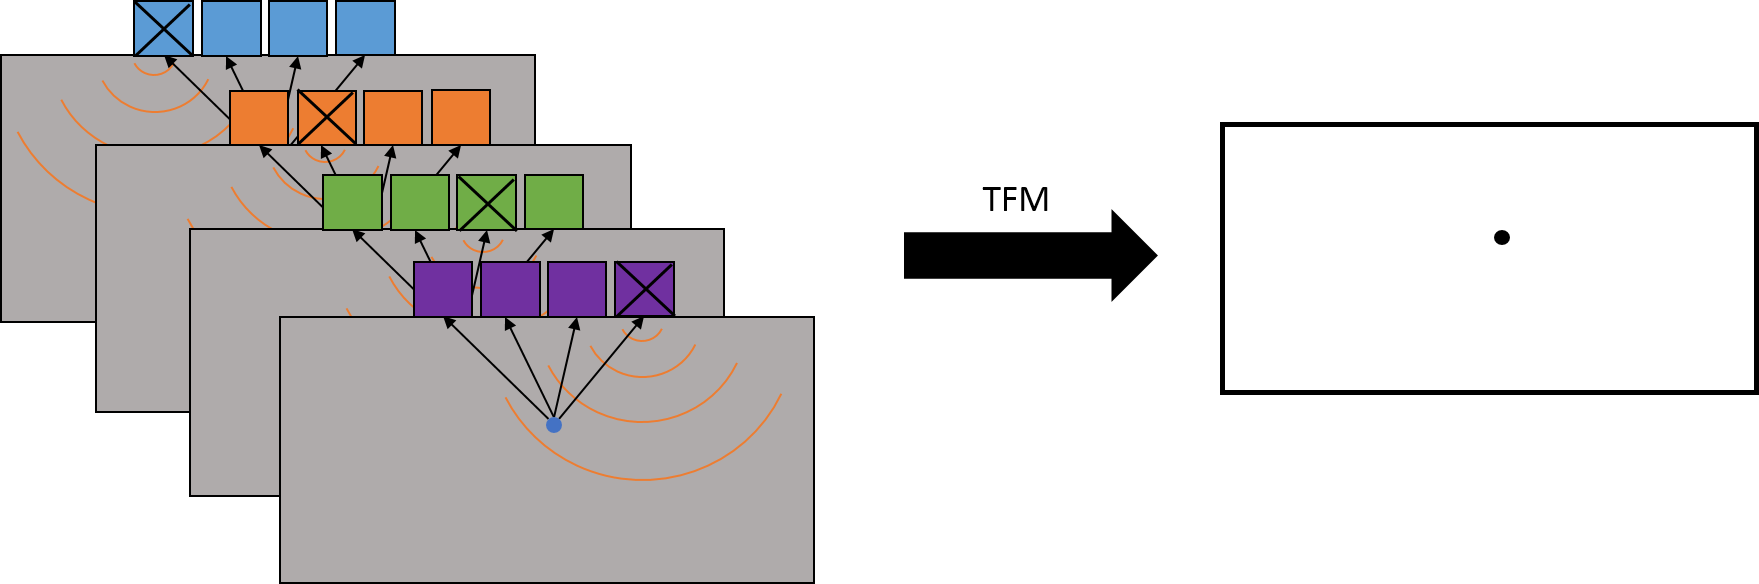
\includegraphics[width=\textwidth]{sactfm1.png}
		\caption{A simple illustration of the TFM imaging algorithm}
		\label{fig:sactfm1}
		\vspace{10mm}
		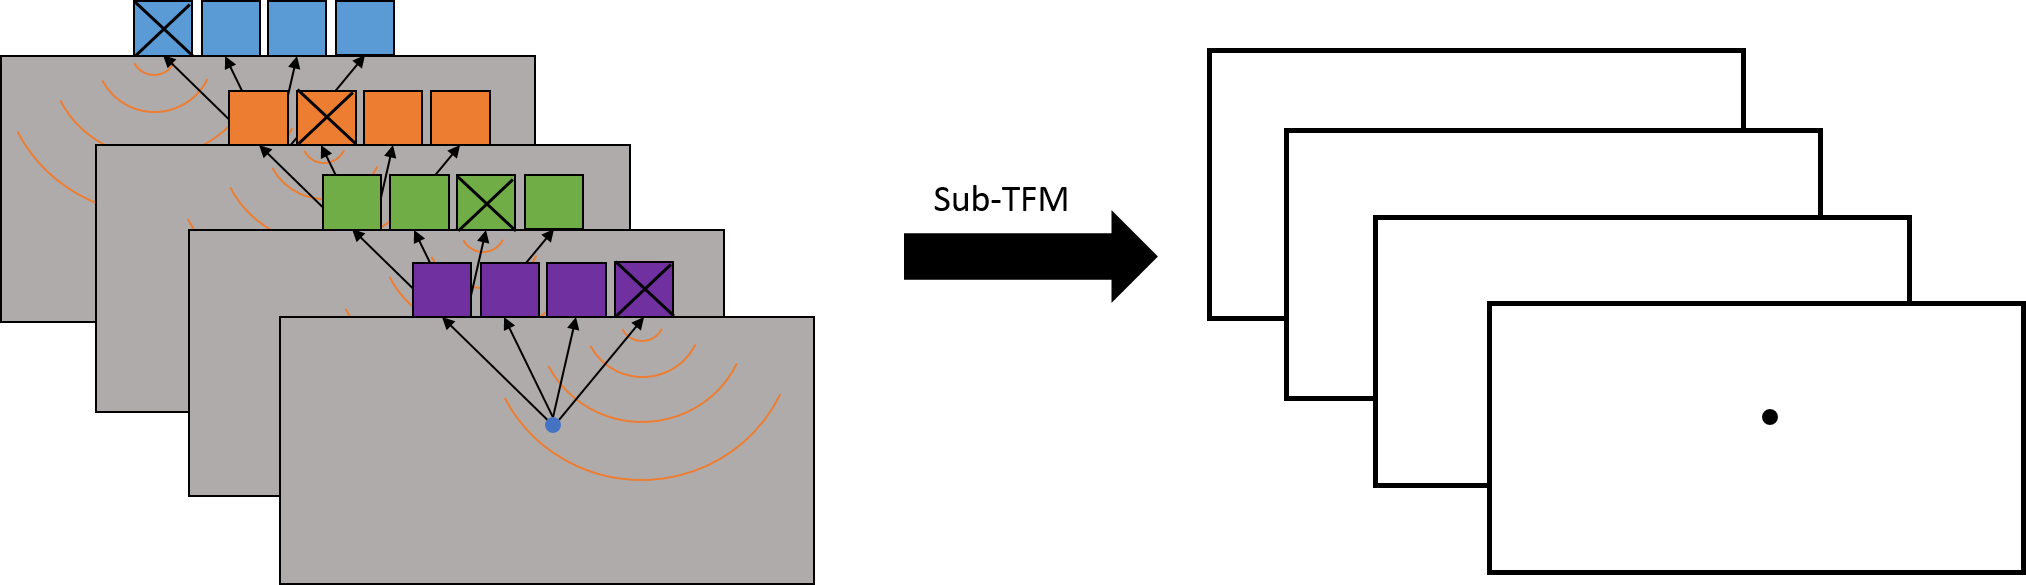
\includegraphics[width=\textwidth]{sactfm2.png}
		\caption{A simple illustration of how Sub-TFM images are generated}
		\label{fig:sactfm2}
		
\end{figure}


In the SASACI process (see Figure~\ref{fig:sac_flowchart}), these Sub-TFM images are summed together to create two new images. One of the ways to do this is to sum all the odd-numbered Sub-TFM images to create the first new image, and all of the even-numbered Sub-TFM images to create the second new image. Section \ref{sec:sasaci_weight} explores methodologies for summing the Sub-TFM images in more detail and proposes a number of differing ways to apply a weighting to the images prior to summation.

\subsection{Cross-Correlation}
Once two differing images are generated, they are input to a cross-correlation function, as shown in Equation~\ref{eq:XCorr}, which generates a matrix of scalars that range between -1 and 1, depending on the level of correlation.

When the images are weighted optimally, any reflections from defects and structural features will be in the same position in each image. Noise from grain structure reflections and multipath propagation will differ between the two images and can therefore be reduced through appropriate signal processing.

In Equation~\ref{eq:XCorr}, $p$ is the resulting cross-correlation matrix. $RX1$ and $RX2$ are the matrices to be cross-correlated and $S$ defines the number of neighbouring pixels to be analysed for one matrix element in the cross-correlation.

 \begin{equation} \label{eq:XCorr}
p(x,y) = \frac{\sum\limits_{i = x - S}^{x+S} \sum\limits_{j = y - A}^{y+S} ( RX1(i,j) \cdot RX2(i,j) )}{\sqrt{\sum\limits_{i = x - S}^{x+S} \sum\limits_{j = y - S}^{y+S} RX1(i,j)^2} \cdot \sqrt{\sum\limits_{i = x - S}^{x+S} \sum\limits_{j = y - S}^{y+S} RX2(i,j)^2}}
 \end{equation}

$S$ can be calculated by the method shown in Equation~\ref{eq:CalcA} and is a measure of the number of pixels used for cross-correlation. $v_L$ is the longitudinal propagation velocity, $c$ is the centre frequency of the array, $l$ distance from the centre of each pixel to analyse in wavelengths, and $\Delta x$ is the pixel pitch of the quantised image measured in meters per pixel. Figure \ref{fig:sasaci_S} shows a graphical representation of the pixels used for the cross-correlation function. $l$ is set to one wavelength in this work.

\begin{figure}[htb]
\centering
		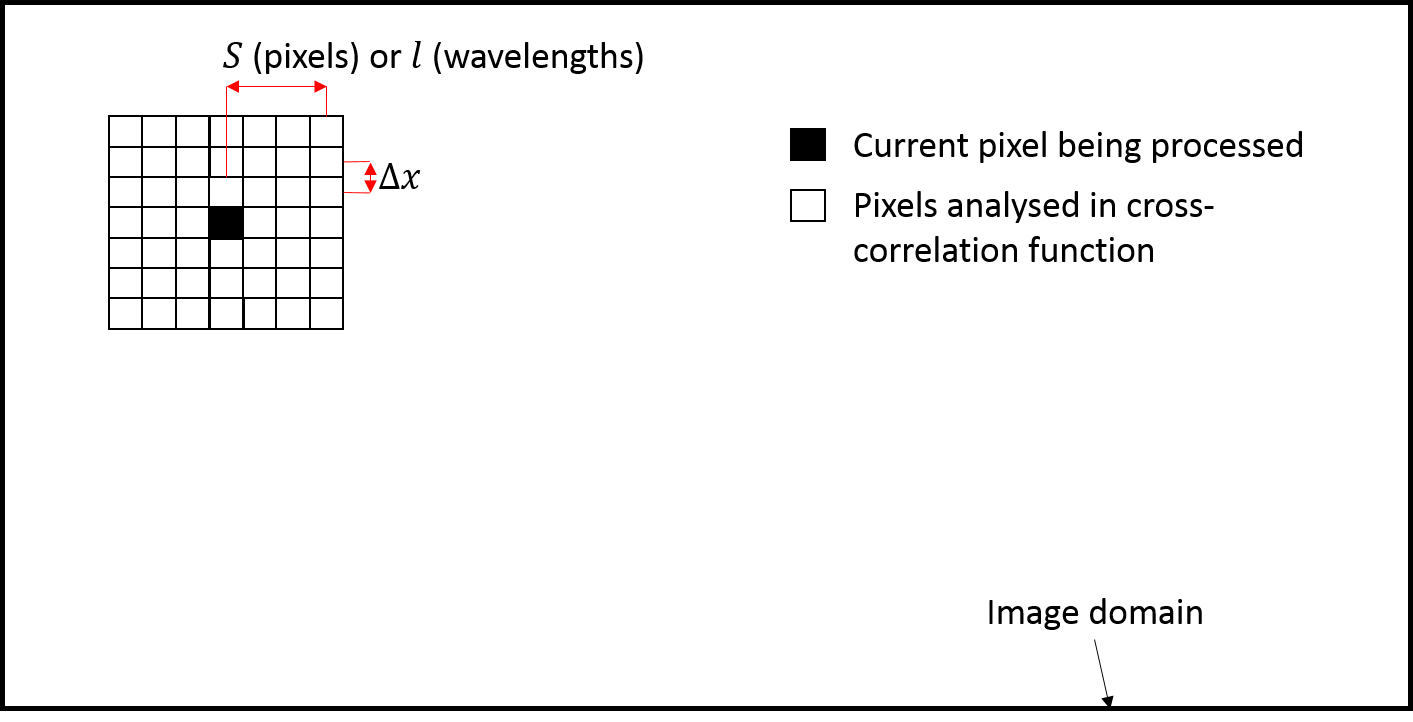
\includegraphics[width=\textwidth]{sacS1.png}
		\caption{A graphical representation of how $S$ is represented for SASACI}
		\label{fig:sasaci_S}
\end{figure}

\begin{equation}\label{eq:CalcA}
S = \frac{v_L \cdot l}{c \cdot \Delta x}
\end{equation}

Thresholding is also applied at this stage, meaning points that are highly uncorrelated will be further minimised, the thresholding equation being shown in Equation~\ref{eq:Threshold}.

\begin{equation} \label{eq:Threshold}
W(x,y) = \begin{cases}
		p(x,y) \cdot{H} , & \text{if }p(x,y) < X\text{;}\\
		p(x,y), & \text{otherwise}.
		\end{cases}
\end{equation}

In Equation~\ref{eq:Threshold}, $W$ is the weighting matrix derived from $p$, the cross-correlation matrix. $X$ is the threshold and $H$ is the weight applied to any pixel whose value is under the threshold. $H$ was set to 0.01 for all of the experimental results presented in this thesis.

Finally, the weighting matrix $W$ is multiplied by the basic TFM image, as shown in Equation~\ref{eq:SASACI} where $SASACI$ is the resultant image.

\begin{equation}\label{eq:SASACI}
SASACI = TFM \cdot W
\end{equation}

 The final SASACI image has the same properties as the TFM image with regards to sensitivity and resolution but should also effectively minimise reflections from sidelobes.

 \section{Experimental Evaluation}

 \subsection{Steel Weld}

 A welded 316L stainless steel sample (Amec Foster Wheeler, UK) was inspected. This sample has a number of defects within the weld and each of these defects was inspected in turn. A photograph of the sample is shown in Figure \ref{fig:amec_1} and a scan of the datasheet detailing the flaws is shown in Figure \ref{fig:amec2}.

\begin{figure}[htb]
\centering
		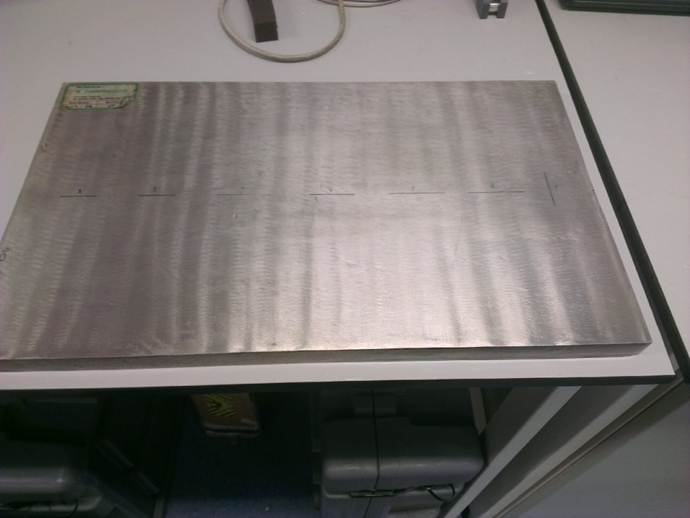
\includegraphics[width=100mm]{AMEC_1.png}
		\caption{A photograph of the welded plate sample}
		\label{fig:amec_1}
\end{figure}

\begin{figure}[p]
\centering
		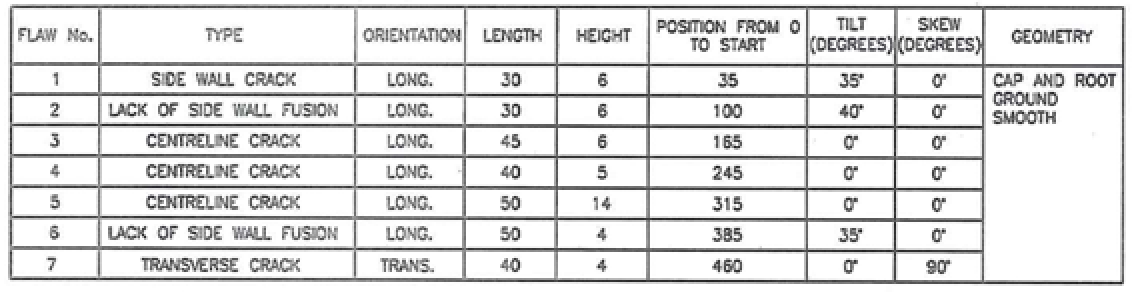
\includegraphics[width=100mm]{AMEC2_1.png}
		
		\vspace{10mm}
		
		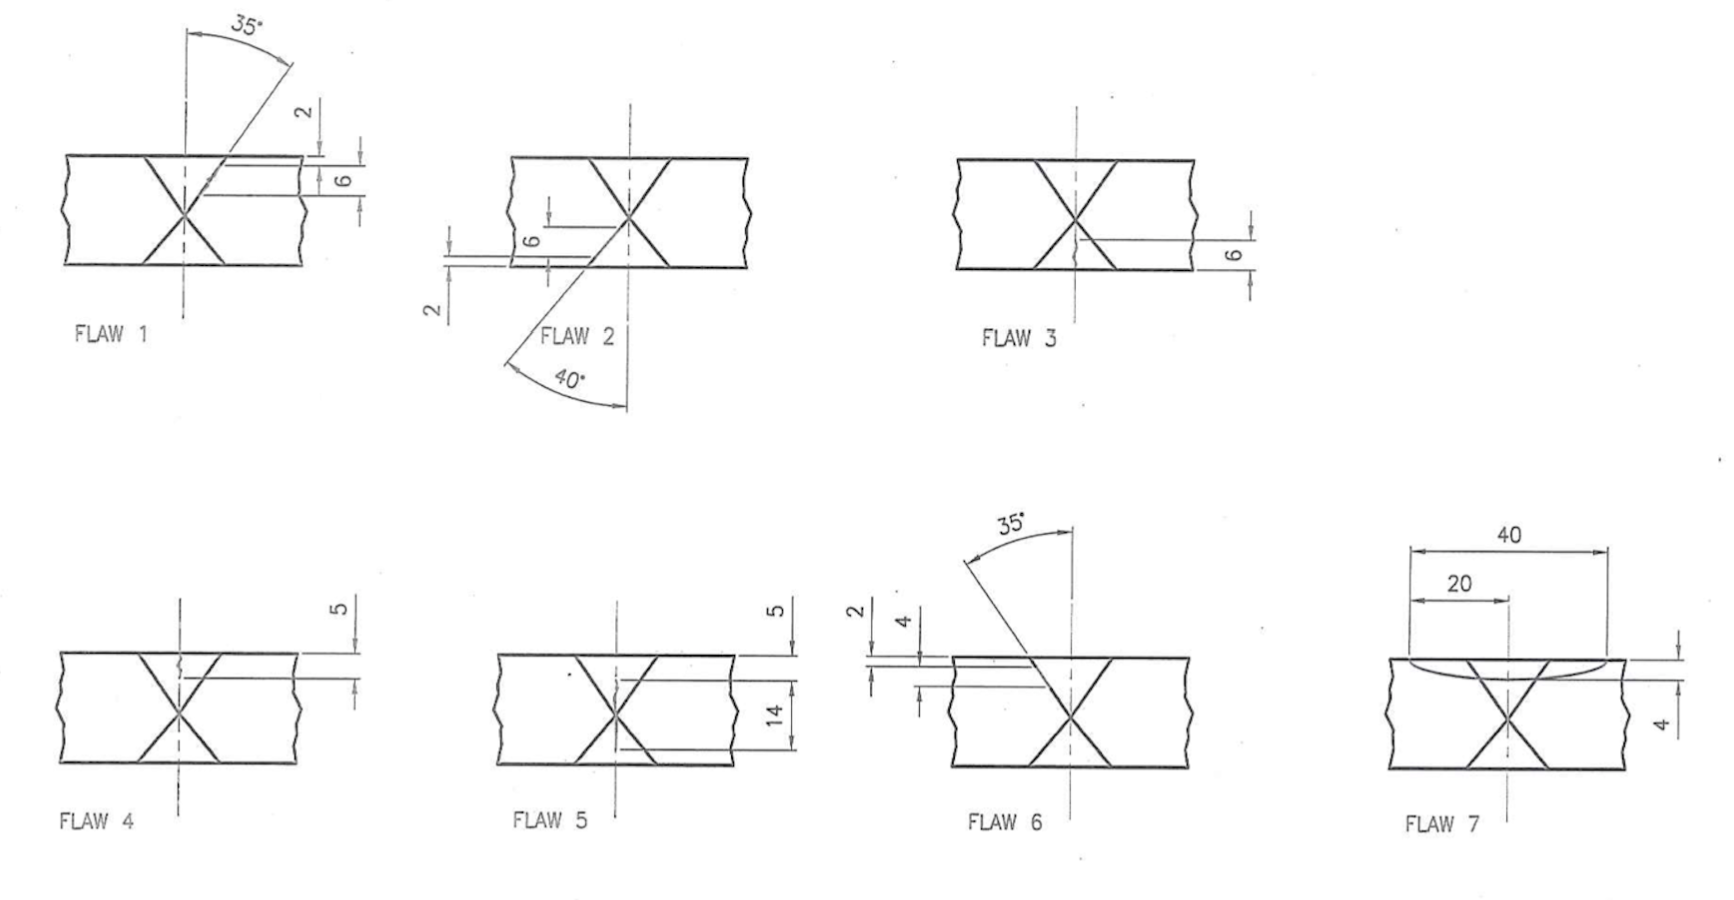
\includegraphics[width=\textwidth]{AMEC12_1.png}
		\caption{Excerpts from the datasheet relating to AMEC's 316L welded sample, showing each defect's type, shape and location within the weld.}
		\label{fig:amec2}
\end{figure}

\subsubsection{Experimental Setup}

Data was collected from this sample using a Dynaray phased array controller (Zetec, USA) and a sub-aperture of a 128 element commercial linear array (Vermon, France). Table \ref{table:amec_setup} shows the parameters used for this experiment.

\begin{table}[htbp!]
\begin{center}
	\begin{tabular}{| c | c |}
	\hline 
	\textbf{Parameter} & \textbf{Value} \\ \hline \hline 
	Array Centre Frequency	& 5 MHz \\ \hline
	Array Aperture & 32 \\ \hline
	Array Pitch & 0.7 mm \\ \hline
	Longitudinal Wave Velocity & 5560 m/s \\ \hline
 	Filter Passband & 0.5 - 10 MHz\\ \hline
	SASACI Threshold & 0.95\\ \hline	
	\end{tabular}
	\caption{Parameters for stainless steel weld inspection}
	\label{table:amec_setup}
	\end{center}
	\end{table}

Due to the sample not being completely flat, it was not possible to directly couple all 128 elements of the array to the sample above each of the defect locations. Instead, a 32 element sub-aperture of the array was used to collect a Full Matrix Capture dataset. For each defect, the array sub-aperture was centred over the defect of interest.

Two defect-free datasets were also recorded; one above the weld and another in a clean, non-welded, region of the stainless steel sample. These were used as baseline to which the other results can be compared.

\subsubsection{Results}

Results from each defect will be presented individually as a series of three images. The leftmost image is the result of the Total Focusing Method on the otherwise unprocessed data. Regions with defects will show the defect location overlaid on this image. The centre image is the TFM result after being applied to the filtered Full Matrix Capture data using the bandpass filter specified in Table \ref{table:amec_setup}. The image on the right is the result of the SASACI process. The input to the SASACI algorithm is a filtered FMC dataset, and the filtered TFM image has been included as a fair comparison between the two methods.

Figure \ref{fig:AMEC_clean} shows the three images from the non-welded area of the stainless steel sample away from the weld. Figure \ref{fig:AMEC_clean_weld} shows the images from the weld, but from a region free of defects.

In these sets of images, the backwall can be seen clearly at a depth of approximately 22mm with no other features in the images. For areas with no defects, it can be observed that SASACI does not offer an improvement compared to TFM on a filtered dataset. This is an expected result as SASACI only tends to improve the images from datasets collected in ultrasonically noisy specimens. Figures \ref{fig:AMEC_flaw1} to \ref{fig:AMEC_flaw7} show the results for defects numbered 1 to 7. These results are presented and discussed in this section.

\begin{figure}[p]
\centering
		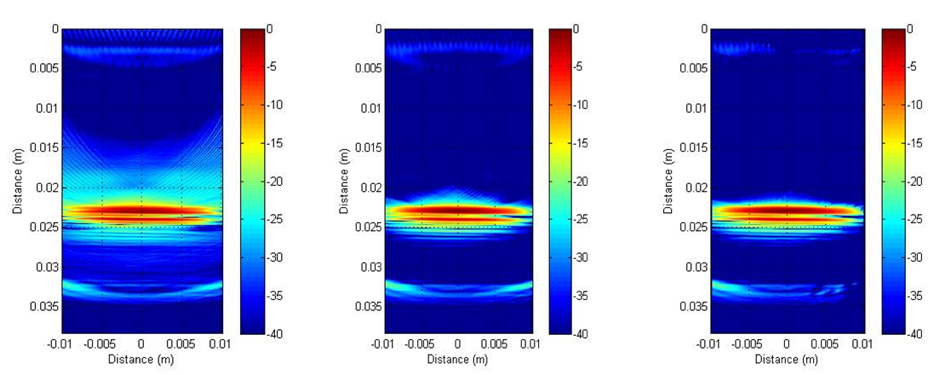
\includegraphics[width=\textwidth]{AMEC3.png}
		\caption{TFM, Filtered TFM and SASACI images of a defect-free, non-welded area of the stainless steel sample.}
		\label{fig:AMEC_clean}
		\vspace{20mm}

		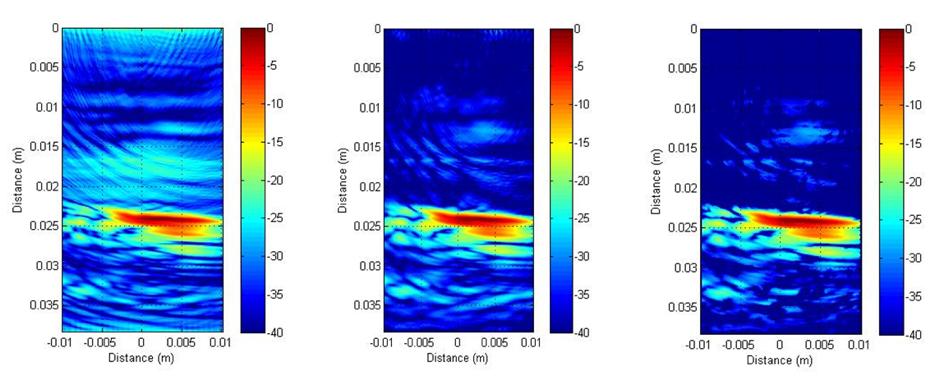
\includegraphics[width=\textwidth]{AMEC4.png}
		\caption{TFM, Filtered TFM and SASACI images of a defect-free area of the weld in the stainless steel sample.}
		\label{fig:AMEC_clean_weld}
\end{figure}

\clearpage
\paragraph{Flaw 1}

Flaw 1 is a side-wall crack angled at 35$^{\circ}$ with respect to the normal. It has a length of 30mm, is 6mm tall and the processed images of this flaw can be seen in Figure \ref{fig:AMEC_flaw1}. The reflection from the flaw is strong and the defect can be seen even in the unfiltered TFM image. As expected, the filtered TFM image reduces a significant portion of the noise and allows the defect to be seen more clearly. The SASACI process reduces this noise (measured by taking the mean amplitude in the highlighted area - this area is consistent throughout the following results) by a further 5dB, though the defect is already visible in the previous image and accurate sizing is possible. 

\vspace{20mm}

\begin{figure}[h!]
\centering
		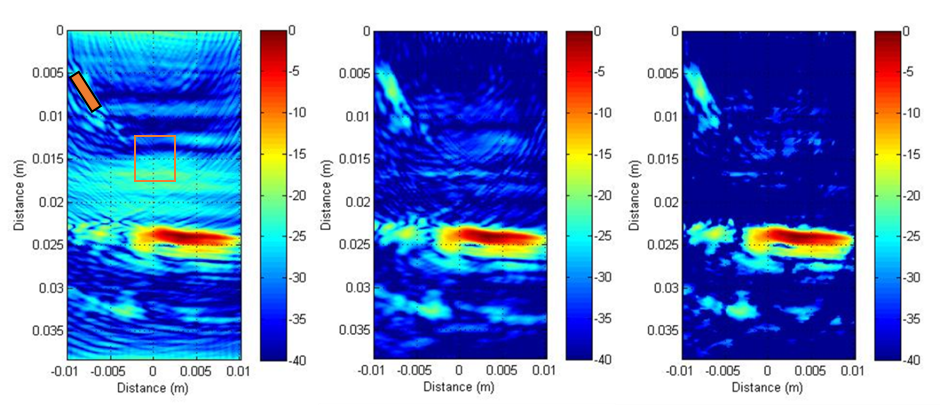
\includegraphics[width=\textwidth]{AMEC5_11.png}
		\caption{TFM, Filtered TFM and SASACI images of Flaw 1 within the stainless steel weld. The side wall crack can be seen clearly at the top left of all three images.}
		\label{fig:AMEC_flaw1}
\end{figure}

\clearpage

\paragraph{Flaw 2}

Flaw 2 is a lack of side wall fusion. It is angled at 40$^{\circ}$ with respect to the normal and has a length and height of 30mm and 6mm respectively. The image results of this flaw are shown in Figure \ref{fig:AMEC_flaw2}. It can be immediately observed from the first of the three images that this section of the weld has much less grain noise compared to the section in which Flaw 1 is located. The background noise level is significantly lower and the defect can be clearly seen. The filtered TFM reduces some of the noise surrounding the backwall and SASACI is able to further reduce some of the noise surrounding the defect.

\vspace{20mm}

\begin{figure}[h!]
\centering
		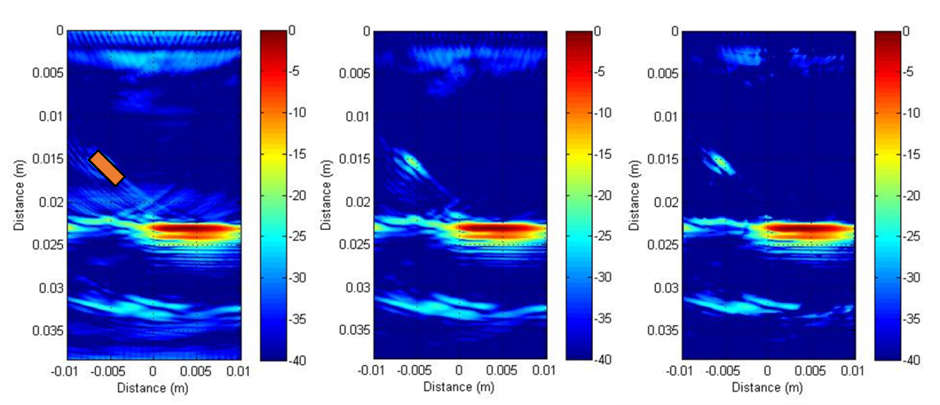
\includegraphics[width=\textwidth]{AMEC6_1.png}
		\caption{TFM, Filtered TFM and SASACI images of Flaw 2 within the stainless steel weld. This defect is a lack of side wall fusion and can be seen approximately 6mm above the back wall on the left hand side of each of the three images.}
		\label{fig:AMEC_flaw2}
\end{figure}

\clearpage

\paragraph{Flaw 3}

Flaw 3 is a vertical centreline crack within the weld. It is 45mm long and 6mm tall. It starts at the bottom of the sample and protrudes upwards. Figure \ref{fig:AMEC_flaw3} shows images of the region in which the flaw is located. No useful information can be observed in the unfiltered TFM image. There is a significant amount of noise surrounding the back wall which hinders analysis of the image. The filtered TFM image reduces noise but it is still not clear where the defect is located. The SASACI image shows further reduced noise, to a point where the top of the defect can be observed. It should be stated that the experimental setup is not optimal for detecting Flaws 3, 4 and 5. To detect vertical flaws, inspection should take place with an angled beam which allows for more energy to be reflected from the defect. A wedge would allow for this.

%\vspace{20mm}

\begin{figure}[h!]
\centering
		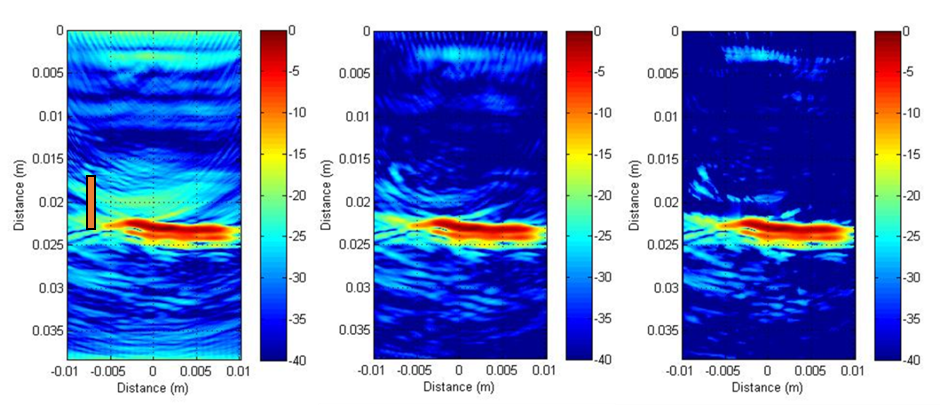
\includegraphics[width=\textwidth]{AMEC7_1.png}
		\caption{TFM, Filtered TFM and SASACI images of Flaw 3 within the stainless steel weld. The centreline crack is expected to be visible in the left hand side of the images and appear as an artefact just above the back wall reflection. It is more prominent in the SASACI image.}
		\label{fig:AMEC_flaw3}
\end{figure}

\clearpage

\paragraph{Flaw 4}

Flaw 4 is also a vertical centreline crack. It is smaller than Flaw 3, being 40mm long and only 5mm tall. This flaw is starts at the top of the sample and protrudes downwards towards the centre of the weld. This flaw cannot be seen in any of the three images shown in Figure \ref{fig:AMEC_flaw4}.

\vspace{20mm}

\begin{figure}[h!]
\centering
		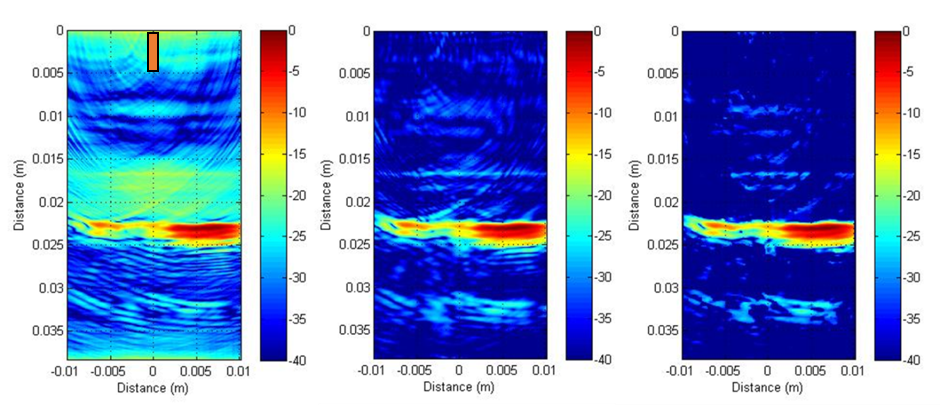
\includegraphics[width=\textwidth]{AMEC8_1.png}
		\caption{TFM, Filtered TFM and SASACI images of Flaw 4 within the stainless steel weld. Flaw 4 is a centreline crack propagating from the top of the weld. Although this defect is not visible in any of the three images, the effects of the crack can be seen as second and third reflections are visible at depths of 8mm and 16mm.}
		\label{fig:AMEC_flaw4}
\end{figure}

\clearpage

\paragraph{Flaw 5}

Flaw 5 is a vertical centreline crack in the centre of the weld. It is larger than the previous flaws and is 50mm in length and 14mm in height. The top of the crack can be seen in the unfiltered TFM image in Figure \ref{fig:AMEC_flaw5}, however the bottom cannot be seen due to the noise around the back wall. The filtered image reduces noise, allowing the top of the crack to be seen clearly. In this case, the bottom of the crack still cannot clearly be seen due to noise. The SASACI image reduces this noise further to a point where the location of the bottom of the crack can be estimated to allow sizing.

\vspace{20mm}

\begin{figure}[h!]
\centering
		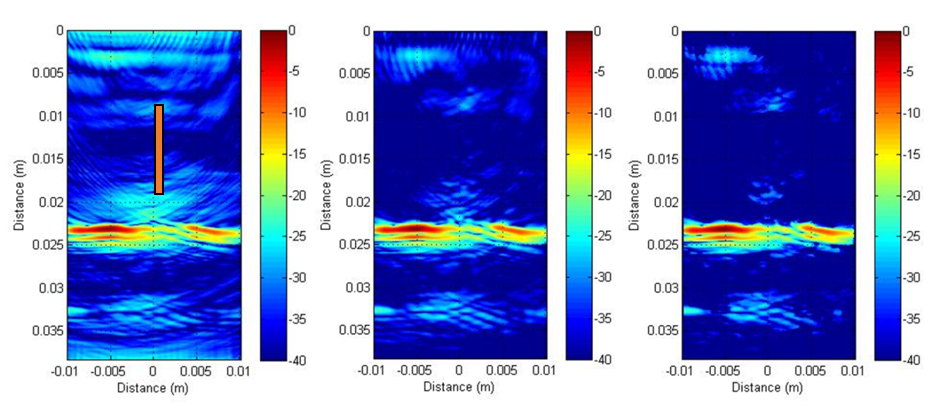
\includegraphics[width=\textwidth]{AMEC9_1.png}
		\caption{TFM, Filtered TFM and SASACI images of Flaw 5 within the stainless steel weld. Flaw 5 is a centreline crack that starts just below the surface and ends just above the back wall of the specimen. The top of the crack can be seen at a depth of 8mm and the bottom is visible at a depth of 20mm. These reflections are most clear in the SASACI image.}
		\label{fig:AMEC_flaw5}
\end{figure}

\clearpage

\paragraph{Flaw 6}

Flaw 6 is a lack of side wall fusion and is at an angle of 35$^{\circ}$ with respect to the normal. The crack is sized 50mm in length and 4mm tall. Figure \ref{fig:AMEC_flaw6} shows the three images related to this defect. The unfiltered TFM image is very noisy due to the grain structure within the weld. The bandpass filtering reduces noise to the point where the defect can be seen above the noise and SASACI further reduces this noise by around 10dB. 

\vspace{20mm}

\begin{figure}[h!]
\centering
		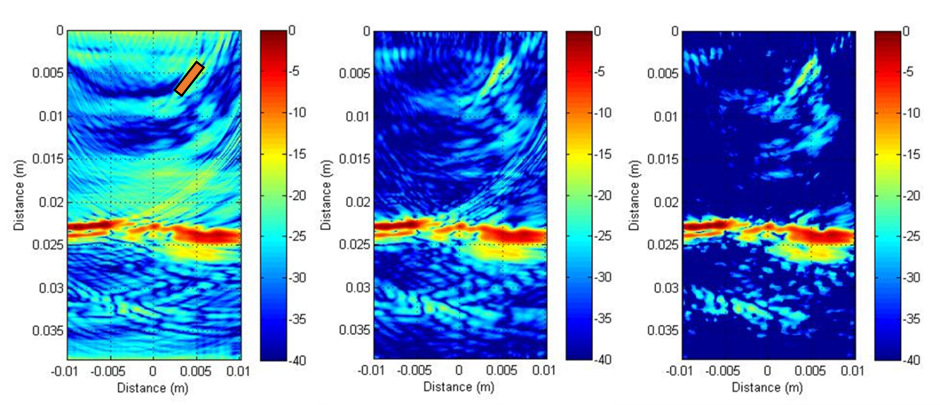
\includegraphics[width=\textwidth]{AMEC10_1.png}
		\caption{TFM, Filtered TFM and SASACI images of Flaw 6 within the stainless steel weld. This defect is a lack of side wall fusion and can be seen at the top-right of both the filtered and SASACI images. The defect is clearest in the SASACI image due to the reduced noise in the image.}
		\label{fig:AMEC_flaw6}
\end{figure}

\clearpage

\paragraph{Flaw 7}

Flaw 7 is a transverse crack at the top of the sample and is 40mm long and 4mm in height. This defect cannot be seen in any of the three images represented in Figure \ref{fig:AMEC_flaw7}. The filtered TFM and SASACI images show clear horizontal artefacts that are also present in Flaw 4. While the defects near the top of the sample cannot be seen in any of the images, it is possible that the flaws are contributing to these artefacts. The orientation of this defect is such that it is expected to be found. There is currently no explanation for the fact that the defect cannot be seen in any of the images.

\vspace{20mm}

\begin{figure}[h!]
\centering
		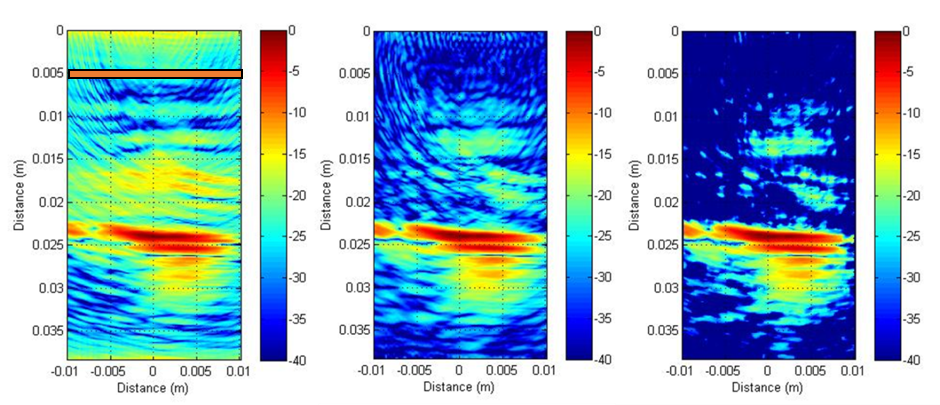
\includegraphics[width=\textwidth]{AMEC11_1.png}
		\caption{TFM, Filtered TFM and SASACI images of Flaw 7 within the stainless steel weld. Flaw 7 is a transverse crack propagating 4mm into the material from the top surface. It is not visible in any of the three images, though the effects can be seen as a large artefact is visible at a depth of around 13mm in both the filtered and SASACI images.}
		\label{fig:AMEC_flaw7}
\end{figure}


\clearpage

\subsection{Dissimilar Weld}

A dissimilar weld specimen (TWI, UK) with implanted flaws was inspected. The specimen is shown in Figure \ref{fig:TWI1}. This specimen has a number of defects, the locations of which can be seen marked on the surface of the sample. In this section only one is investigated for the evaluation of this algorithm. 

\begin{figure}[h!]
\centering
		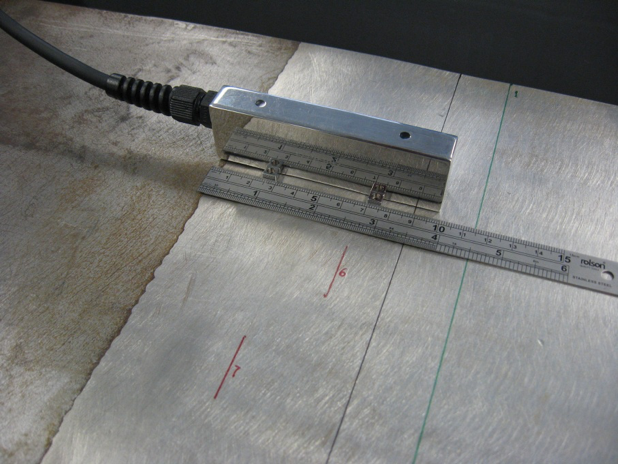
\includegraphics[width=100mm]{TWI1.png}
		\caption{A dissimilar weld specimen}
		\label{fig:TWI1}
\end{figure}

\subsubsection{Experimental Setup}

The defect focused upon for this experiment was a 20mm long vertical crack that began approximately 35mm from the top of the sample, protruding downwards.

A commercial 128 element linear 5MHz array (Vermon, France) was used to record an FMC dataset using a 45 element sub-aperture of the array. A sub-aperture was used because, similar to the previous experiment, the specimen was not flat and a contact inspection using the full aperture of the array was not possible. The array was driven by a Dynaray phased array controller (Zetec, USA). Table \ref{table:twi_setup} shows additional experimental parameters.

\begin{table}[htbp!]
\begin{center}
	\begin{tabular}{| c | c |}
	\hline 
	\textbf{Parameter} & \textbf{Value} \\ \hline \hline 
	Array Centre Frequency	& 5 MHz \\ \hline
	Array Aperture & 45 \\ \hline
	Array Pitch & 0.7 mm \\ \hline
	Longitudinal Wave Velocity & 5700 m/s \\ \hline
 	Filter Passband & N/A \\ \hline
	SASACI Threshold & 0.95\\ \hline	
	\end{tabular}
	\caption{Parameters for stainless dissimilar weld inspection}
	\label{table:twi_setup}
	\end{center}
	\end{table}

\subsubsection{Results}

The Full Matrix Capture dataset was input to both the TFM and SASACI algorithms and the results compared. The TFM and SASACI results are shown in Figures \ref{fig:TWI2} and \ref{fig:TWI3} respectively. The images are shown with a 30dB dynamic range. The SNR was measured in each of these images. The signal was defined as the area where the back wall and extremities of the crack were expected to be, and the noise was defined as all other areas. Table \ref{table:twi} shows the calculated signal to noise ratio for each of the algorithms. 

\begin{figure}[p!]
\centering
		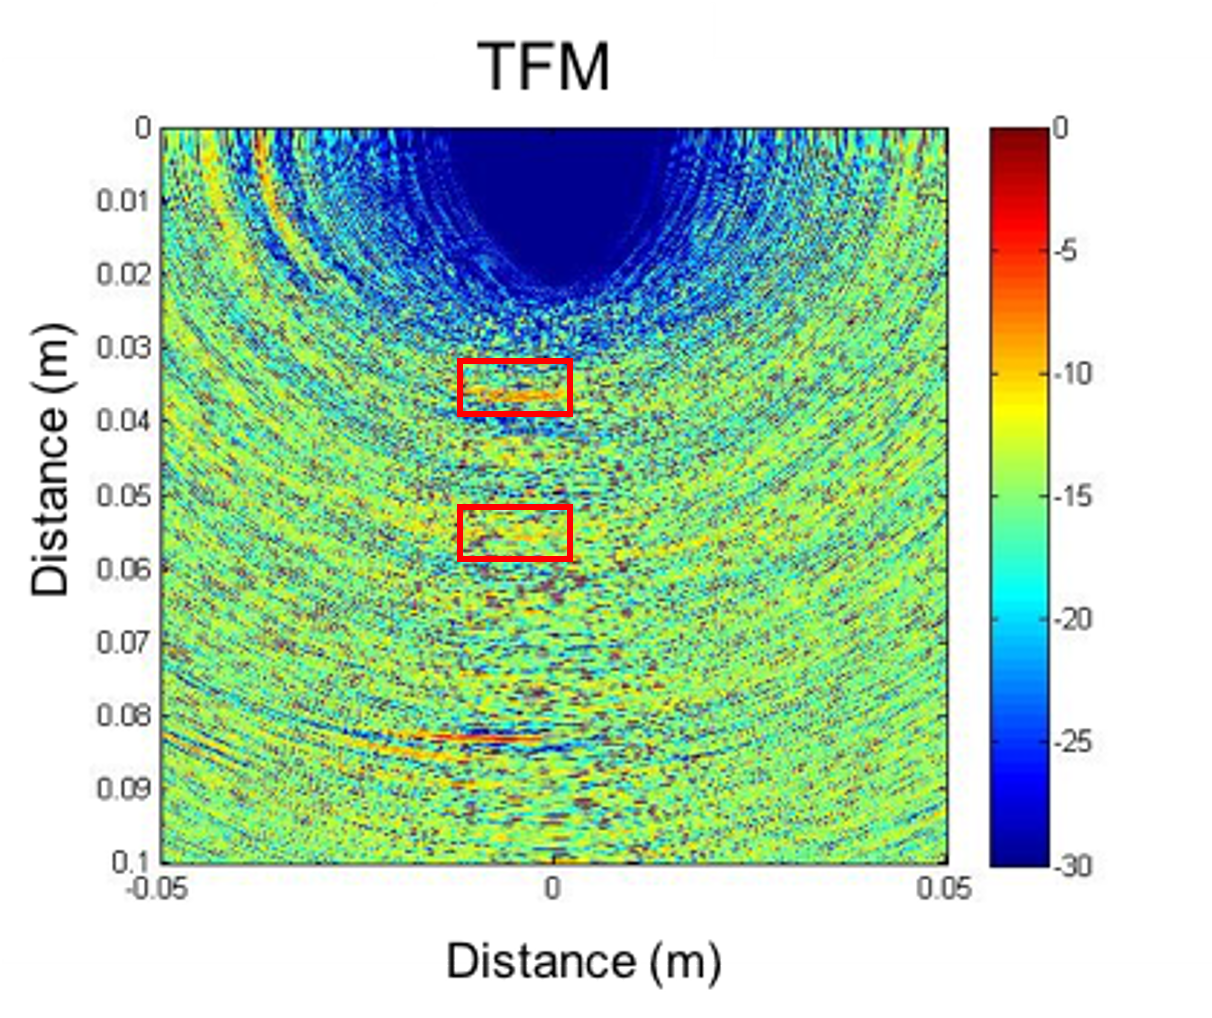
\includegraphics[width=100mm]{TWI2_1.png}
		\caption{TFM result from the dissimilar weld specimen. The region where the reflections from the top and bottom of the crack are expected to appear are highlighted in red.}
		\label{fig:TWI2}

		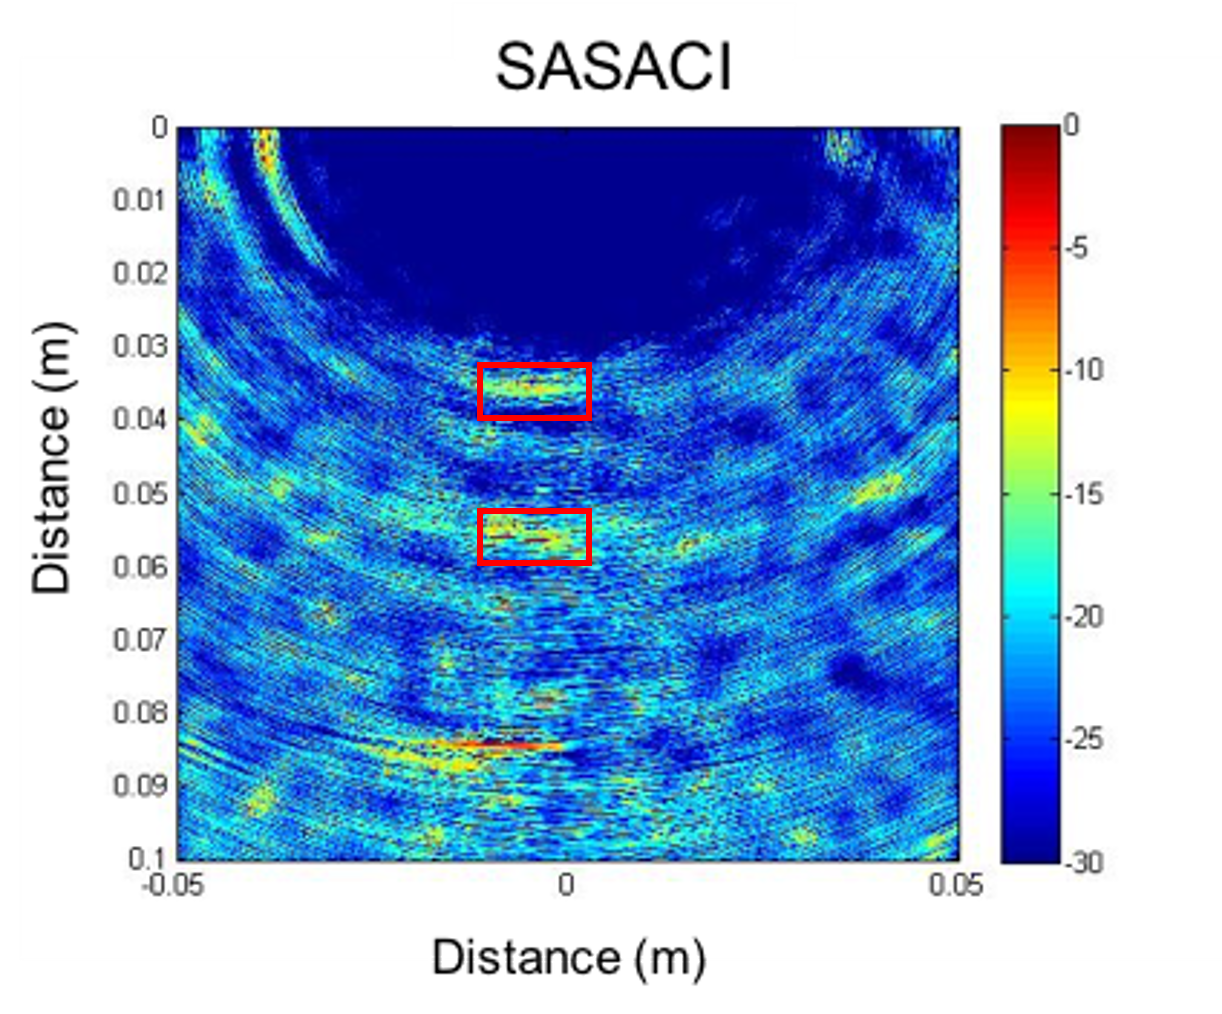
\includegraphics[width=100mm]{TWI3_1.png}
		\caption{SASACI result from the dissimilar weld specimen. The region where the reflections from the top and bottom of the crack are expected to appear are highlighted in red.}
		\label{fig:TWI3}
\end{figure}

\begin{table}[h!]
\begin{center}
	\begin{tabular}{| c | c |}
	\hline 
	\textbf{Algorithm} & \textbf{SNR} \\ \hline \hline 
	TFM	& 7 dB\\ \hline
	SASACI & 20 dB\\ \hline
	\end{tabular}
	\caption{Signal to Noise Ratio for the dissimilar weld sample}
	\label{table:twi}
	\end{center}
	\end{table}

In each of the images, the back wall can be clearly seen at a depth of 85mm. The top of the vertical crack can also be seen in both the TFM and SASACI images, at a depth of 35mm and centred. The SASACI algorithm reduces the background noise of the image to the point where the bottom of the crack can also be observed. This is visible at a depth of 55mm in the SASACI image and is not visible in the TFM image. These regions have been highlighted via a red rectangle in each of the images.

Although the noise is greatly reduced in the SASACI image, there are a number of remaining areas with an amplitude response close to that of the defect. Tuning of the SASACI parameters may reduce the amplitude of these indications.

\section{Apodisation Analysis}\label{sec:sasaci_weight}

In this section, different apodisation methods will be evaluated using results from experimental data to fine-tune the parameters of the algorithm. Five different apodisation techniques were trialled and used to weight an FMC dataset in order to create different sets of sub-TFM images. 

\subsection{Experimental Setup}\label{sec:sasaci_siemens}

The SASACI algorithm was implemented in CUDA C++ running on NVidia graphics cards using the efficient imaging methods described in Chapter \ref{chap:cuetfm}. An Inconel 625 step wedge was provided by Siemens (via E.ON) for these tests. An image of the specimen is shown in Figure~\ref{fig:step_wedge}.

\begin{figure}[htbp]
\centering
		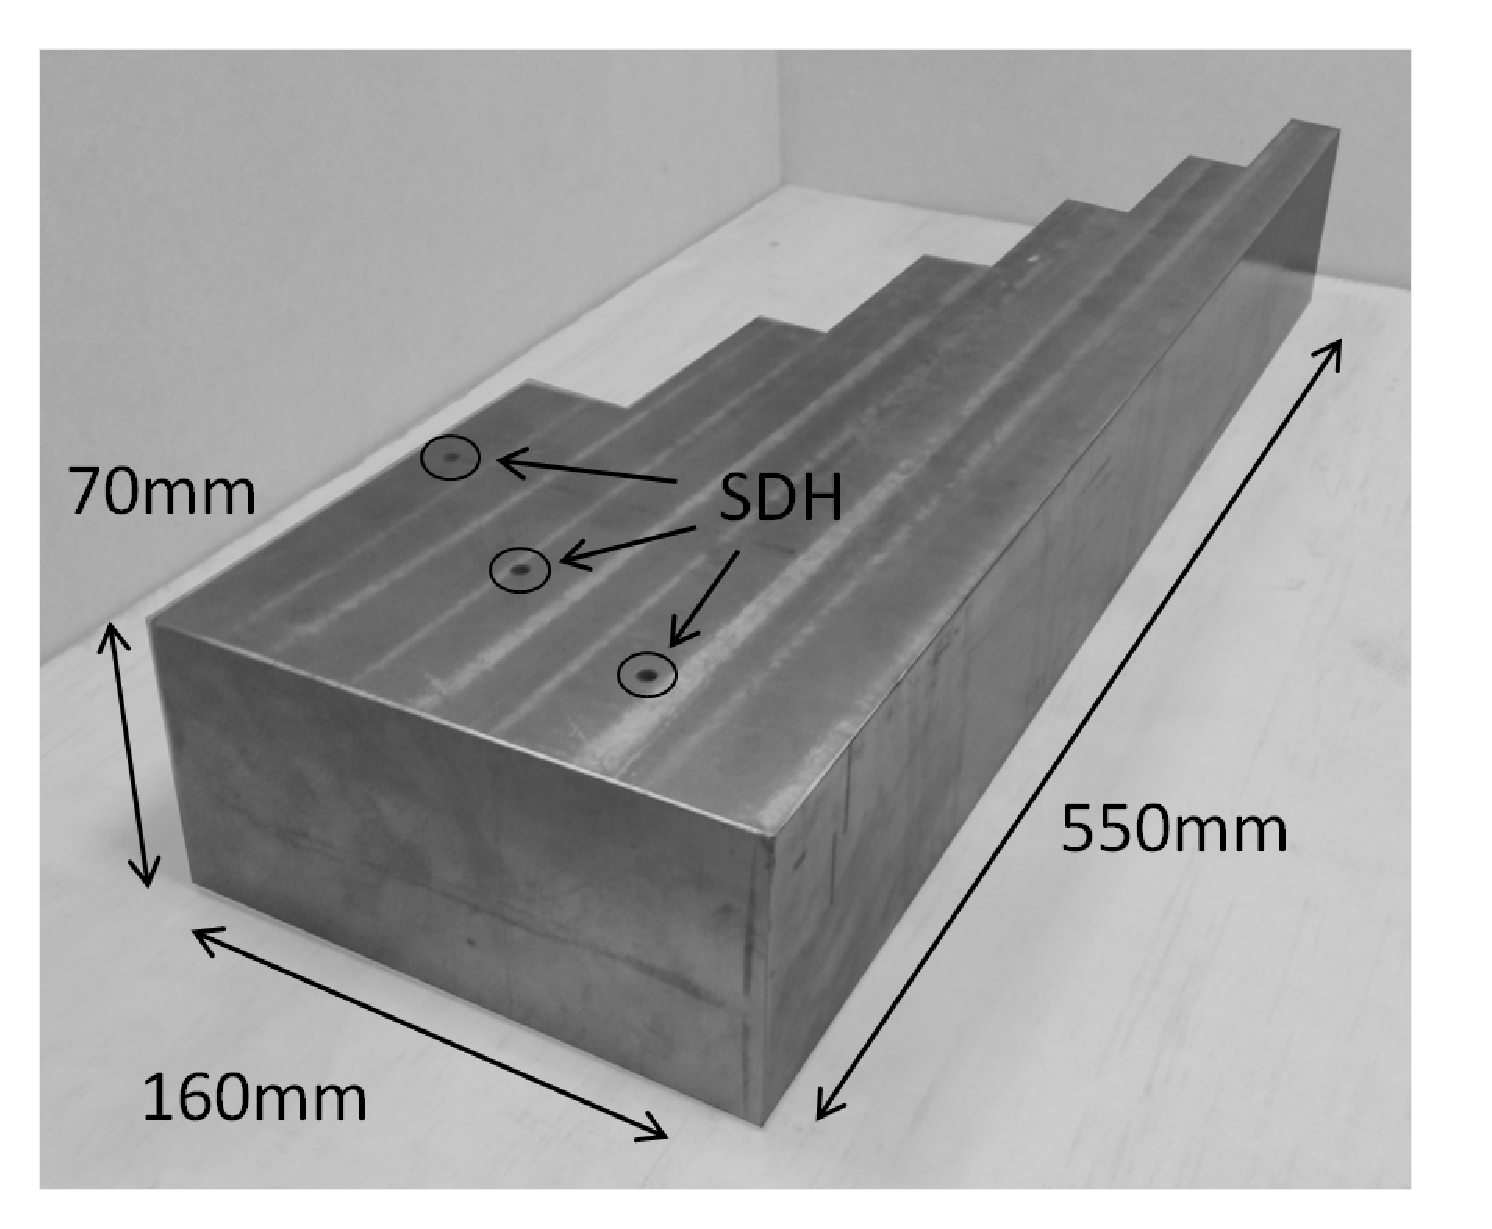
\includegraphics[width=100mm]{StepWedge.eps}
		\caption{Inconel 625 Specimen}
		\label{fig:step_wedge}
\end{figure}

A commercial array (Vermon, France) was used to record ultrasonic data. The parameters are shown in Table~\ref{table:vermon_5mhz}. The array was driven with a Dynaray phased array controller (Zetec, USA). The Dynaray's set-up parameters are shown in Table~\ref{table:dynary_setp}. 

\begin{table}[htbp!]
\begin{center}
	\begin{tabular}{| c | c |}
	\hline 
	\textbf{Parameter} & \textbf{Value} \\ \hline \hline 
	Pulse Voltage	&  50 V \\ \hline
	Hardware Gain & 40dB \\ \hline
	Pulse Width & 140 ns \\ \hline
	Sampling Frequency & 100 MHz \\ \hline
	\end{tabular}
	\caption{Dynaray setup parameters for step wedge inspection}
	\label{table:dynary_setp}
	\end{center}
	\end{table}
	
Due to the size of the sample, it is not possible to generate an image from a single scan that shows all of the sample's features. Instead, a single feature will be selected. The feature that the experimental results will concentrate upon is the Side Drilled Hole (SDH) that is at a depth of 60mm from the top of the specimen. This is the middle hole in Figure \ref{fig:step_wedge}.

The FMC dataset also had a bandpass filter applied to remove noise in the pre-processing state. The applied filter was a second order Butterworth bandpass filter with -3dB cut-offs at 2MHz and 6MHz. A Butterworth filter was chosen due to its flat frequency response in the passband.

\subsection{Experiment and Results}\label{sec:sasaci_apodization}
\subsubsection{Benchmark TFM}
The resultant image from the experiment defined above is shown in Figure~\ref{fig:TFM} with a dynamic range of 40dB.
\begin{figure}[htbp]
\centering
		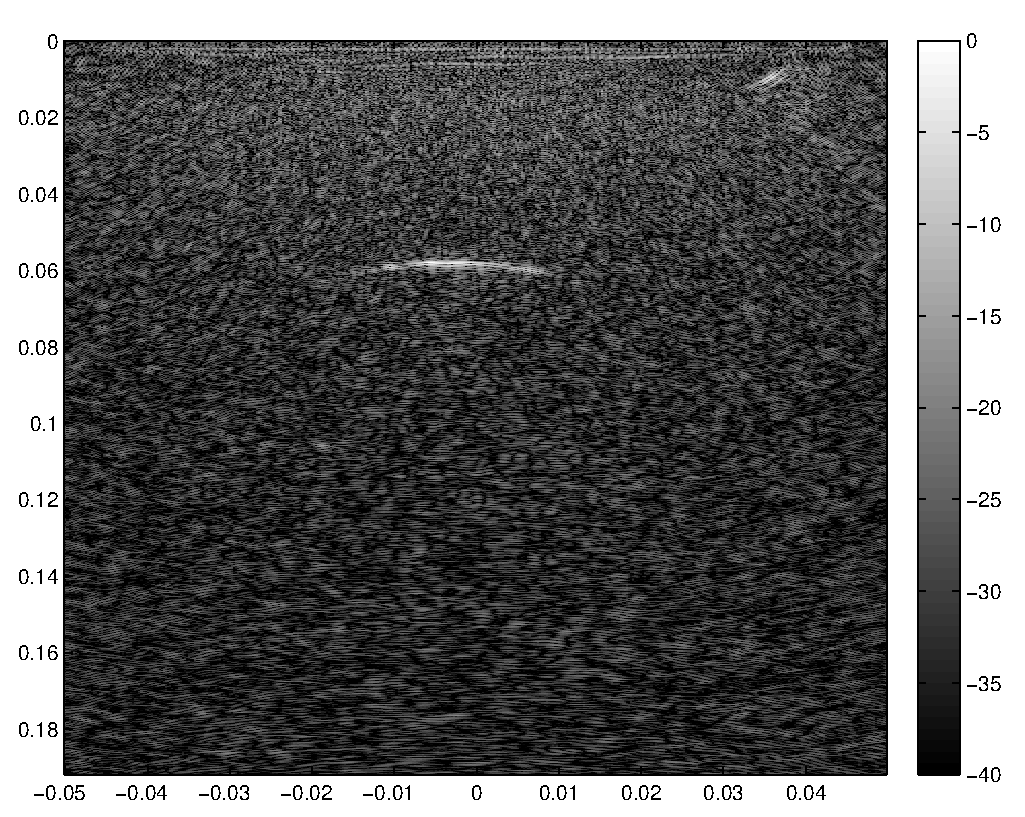
\includegraphics[width=100mm]{TFM.eps}
		\caption{A Conventional TFM Image}
		\label{fig:TFM}
\end{figure}
In Figure~\ref{fig:TFM}, the SDH is central and is at a depth of 60mm. Due to multipath propagation and the fact that the speed of sound is not constant in the material, the hole appears as a line in the image. This is a limitation of the imaging process that SASACI cannot overcome. It is evident that the longitudinal propagation velocity is set correctly, as another SDH can be seen in Figure \ref{fig:TFM} at a depth of 10mm. This feature is resolved correctly in the image due to the fact that is is close to the surface and the sound energy has less distance to travel and therefore less opportunity for error to be accumulated in estimating the distance travelled.

There are a number of different ways to weight the sub-TFM images before combining them. Seo and Yen\cite{seo_sidelobe_2008} investigated four methods of doing this for a one-dimensional cross-correlation approach. Each of the approaches, as well as a novel hamming windowing approach, will be evaluated for the current methodology. The Hamming window is designed to reduce the amplitude of the sidelobe closest to the main lobe, but at the expense of the rest of the side lobes being much higher when compared to a Hann window.

For the SASACI processing a number of variables need to be set, as described in Section \ref{sec:sasaci}. These values are defined in Table~\ref{table:sasaci_params} and remain constant in all the results presented in this Chapter. The value of A was chosen to compare 2 wavelengths of data for the cross-correlation algorithm. Multiple values of $H$ and $T$ were investigated. The values in Table~\ref{table:sasaci_params} were used in this experiment as they produce an optimal image. Future work will involve generating an adaptive processing methodology to set these values algorithmically.

\begin{table}[htbp!]
\begin{center}
	\begin{tabular}{| c | c |}
	\hline 
	\textbf{Parameter} & \textbf{Value} \\ \hline \hline 
	X	&  0.9 \\ \hline
	H & 0.1 \\ \hline
	S & 6 \\ \hline
	l & 1 \\ \hline
	\end{tabular}
	\caption{SASACI Parmeters}
	\label{table:sasaci_params}
	\end{center}
	\end{table}
	
\subsubsection{Alternating Elements Apodisation}
Figure~\ref{fig:apod_alt} shows the weighting applied to the transmitting elements to create the modified aperture. Although 32 elements are shown, any number of elements can be used with this method and the pattern expanded or reduced as necessary. In this experiment, a 128 element array was used and the weighting shown is simply repeated as necessary.

The SASACI image after using the weighting shown in Figure~\ref{fig:apod_alt} is shown in Figure~\ref{fig:apod_alt_result}. Compared to the TFM image there is reduced speckle noise and the second, shallow SDH appears clearer.

\subsubsection{Hamming Window Apodisation}
Hamming windowing is an apodisation technique untested by Seo and Yen, but is thought to have potentially improved results due to it being designed to reduce the nearest sidelobe to the main lobe. The hamming window weightings are shown in Figure~\ref{fig:apod_ham} and the resultant SASACI image in Figure~\ref{fig:apod_ham_result}.

\subsubsection{Hann Window Apodisation}
Compared to the Hamming window, the Hann windowing function has a much steeper frequency roll-off and will therefore minimise sidelobes. The Hann window weightings are shown in Figure~\ref{fig:apod_han} and the results from this apodisation method shown in Figure~\ref{fig:apod_han_results}.

\subsubsection{Common Midpoint Apodisation}

Figure~\ref{fig:apod_com} shows the apertures used for the common midpoint apodisation. Essentially, the two apertures have a number of elements disabled at opposing sides. This is done to create a pair of images where the position and amplitude of noise differs between them. The result image is depicted in Figure~\ref{fig:apod_com_result}. 

\subsubsection{Random Element Apodisation}
The random element apodisation weighting is shown in Figure~\ref{fig:apod_ran}. This method has the limitation of yielding differing results each time the random element permutations are chosen. Is is possible to generate permutations over and over until an preferred set of elements are found and this research could be completed in future. A random (non-optimised) result is shown in Figure~\ref{fig:apod_ran_result}

\begin{figure}[p]
\centering
		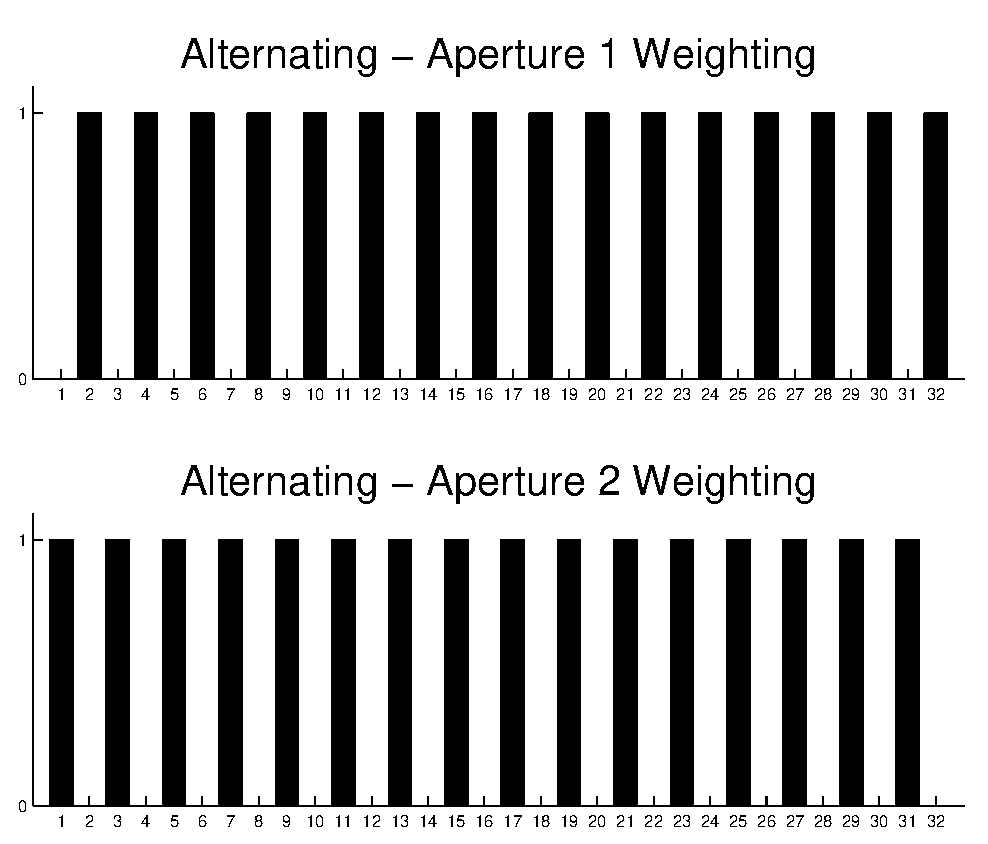
\includegraphics[width=100mm]{Alternating.eps}
		\caption{Alternating Apodisation}
		\label{fig:apod_alt}

		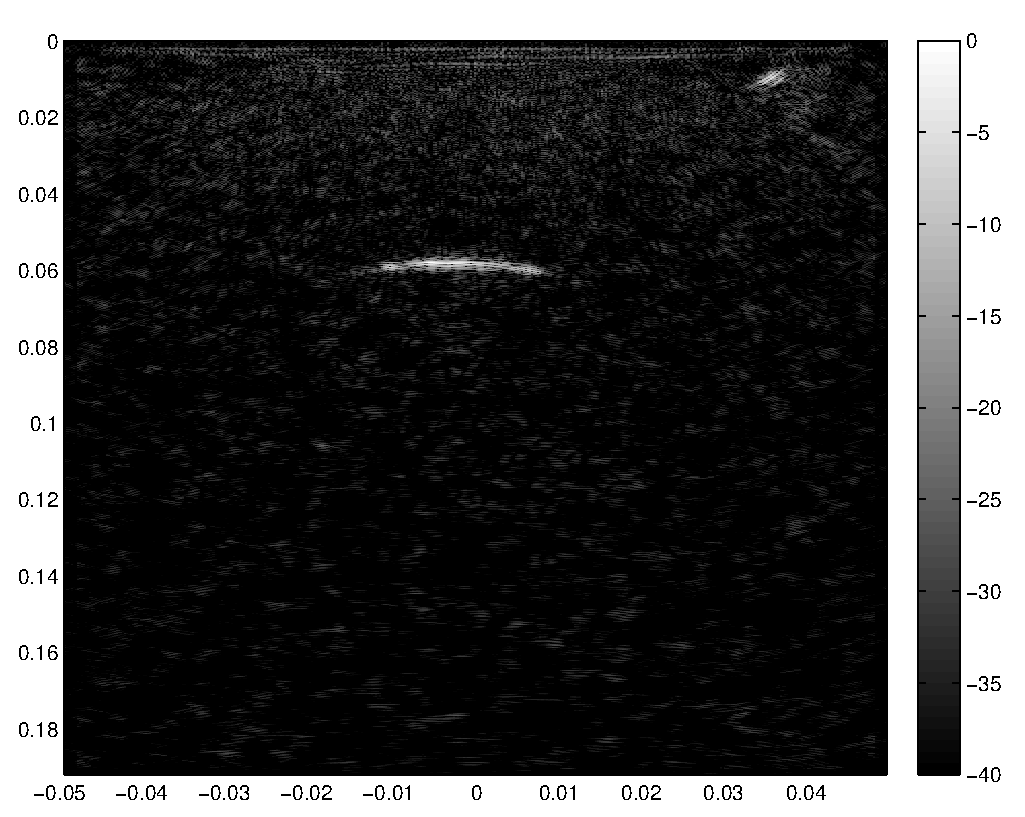
\includegraphics[width=100mm]{SAC_Alternating.eps}
		\caption{Alternating Apodisation SASACI Result}
		\label{fig:apod_alt_result}
\end{figure}

\begin{figure}[p]
\centering
		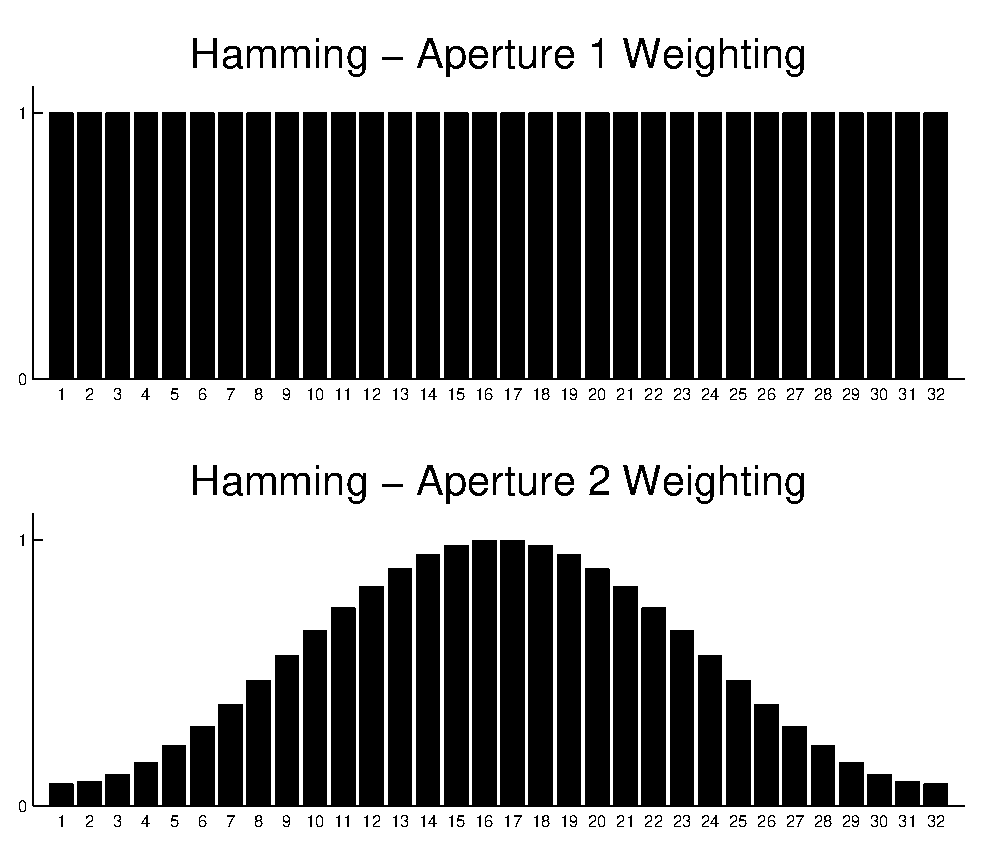
\includegraphics[width=100mm]{Hamming.eps}
		\caption{Hamming Apodisation}
		\label{fig:apod_ham}

		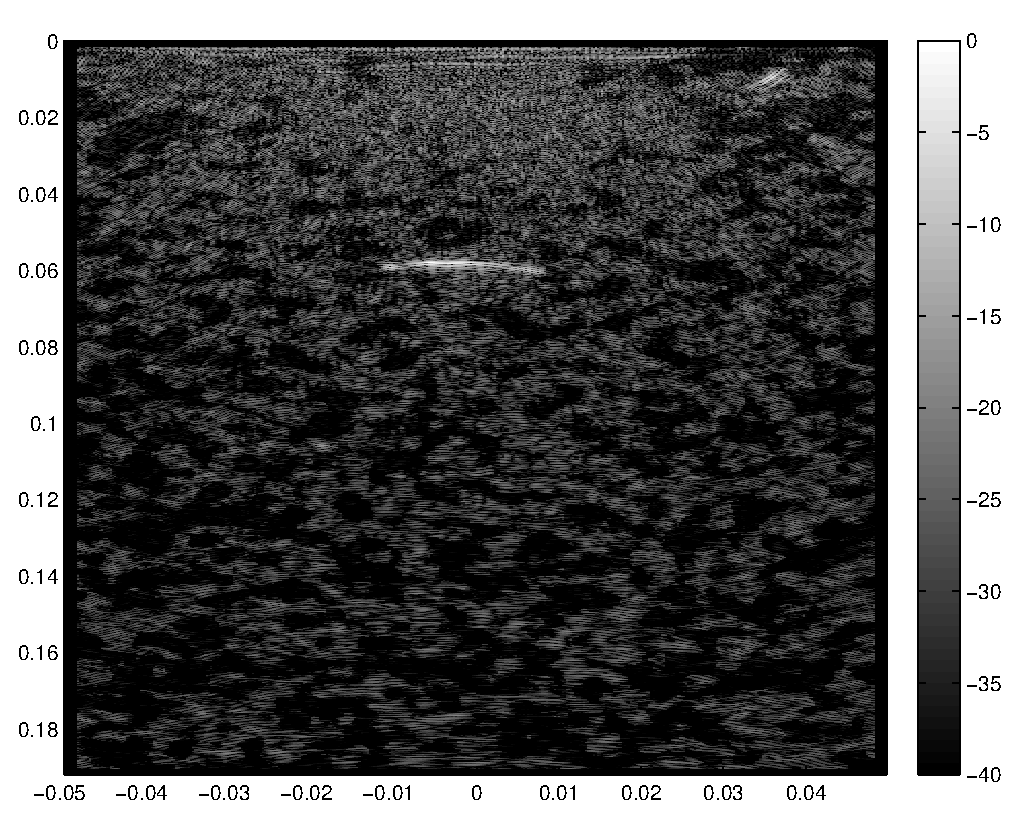
\includegraphics[width=100mm]{SAC_Hamming.eps}
		\caption{Hamming Apodisation Result}
		\label{fig:apod_ham_result}
\end{figure}

\begin{figure}[p]
\centering
		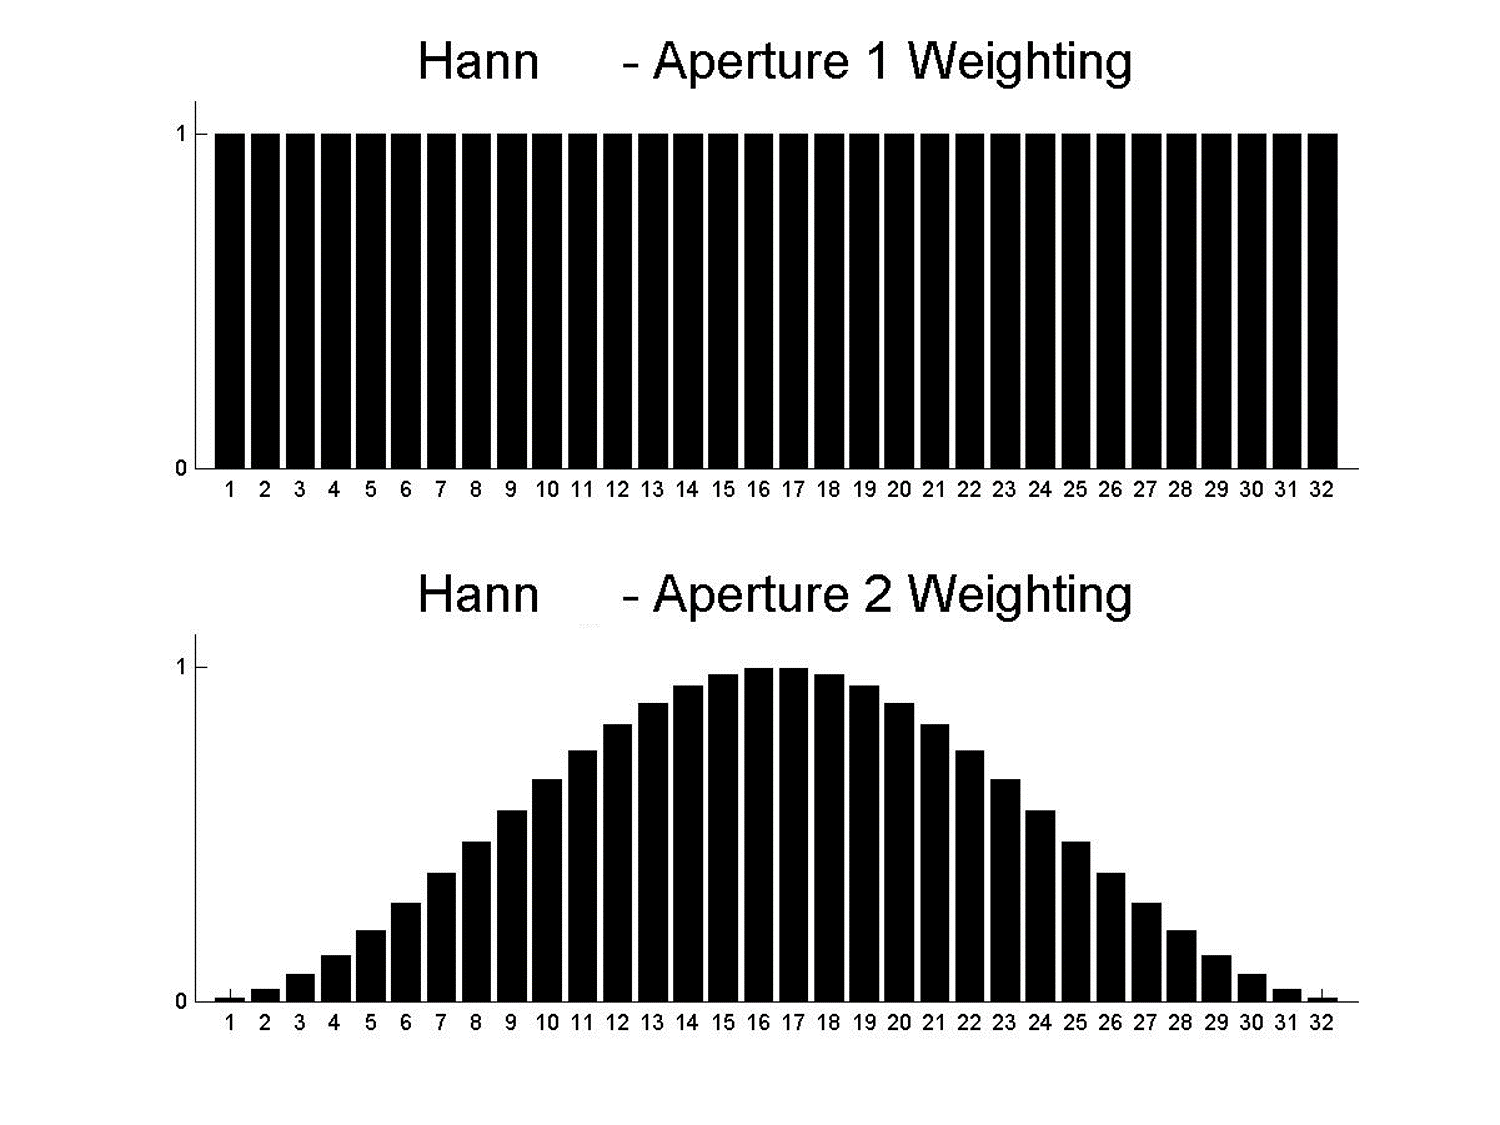
\includegraphics[width=100mm]{Hanning.png}
		\caption{Hann apodisations}
		\label{fig:apod_han}

		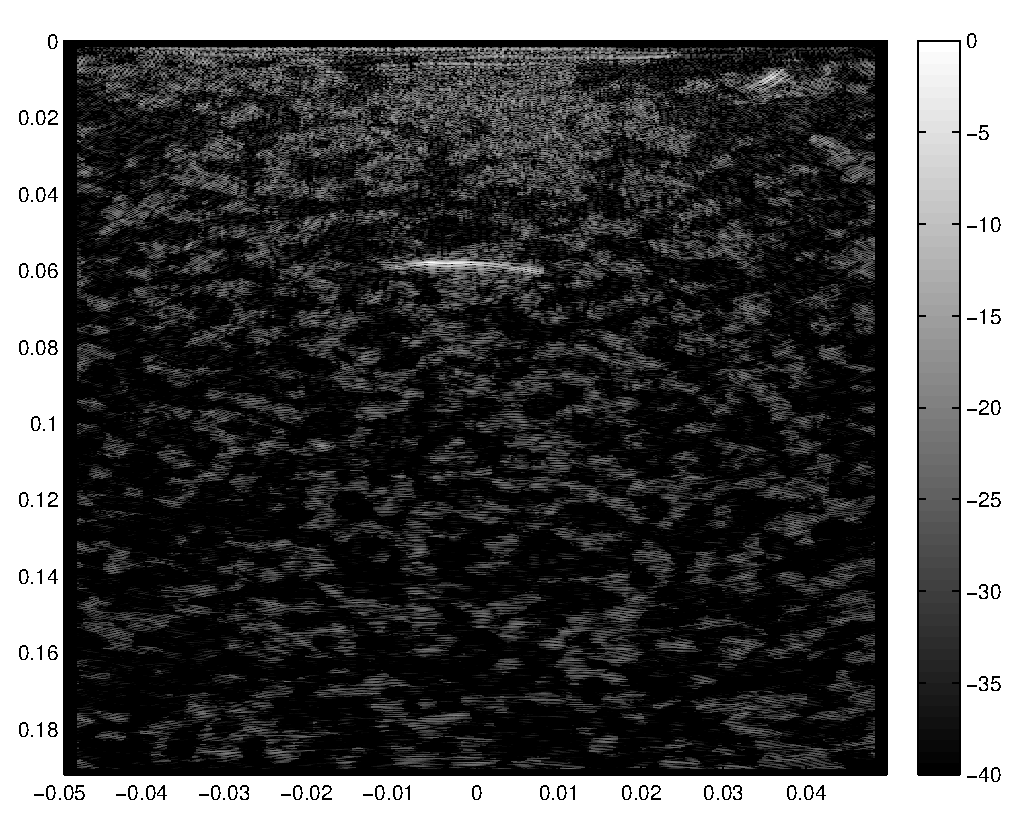
\includegraphics[width=100mm]{SAC_Hanning.eps}
		\caption{Hann apodisations}
		\label{fig:apod_han_results}
\end{figure}

\begin{figure}[p]
\centering
		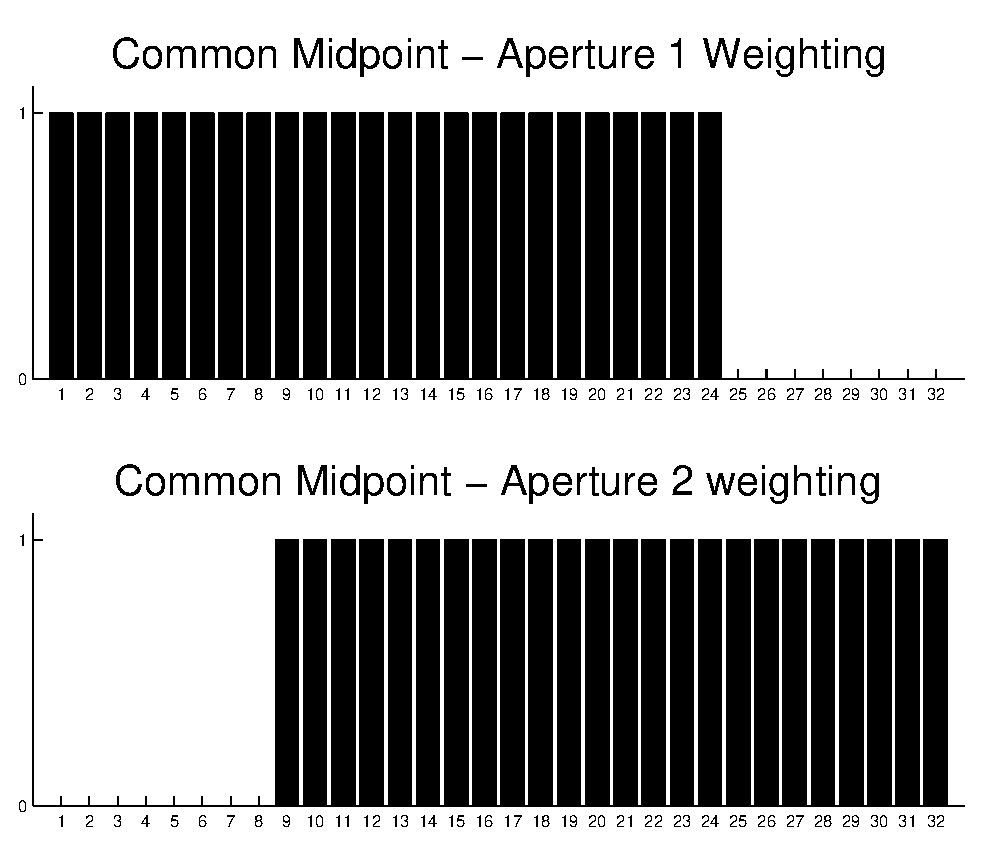
\includegraphics[width=100mm]{Common.eps}
		\caption{Common Apodisation}
		\label{fig:apod_com}

		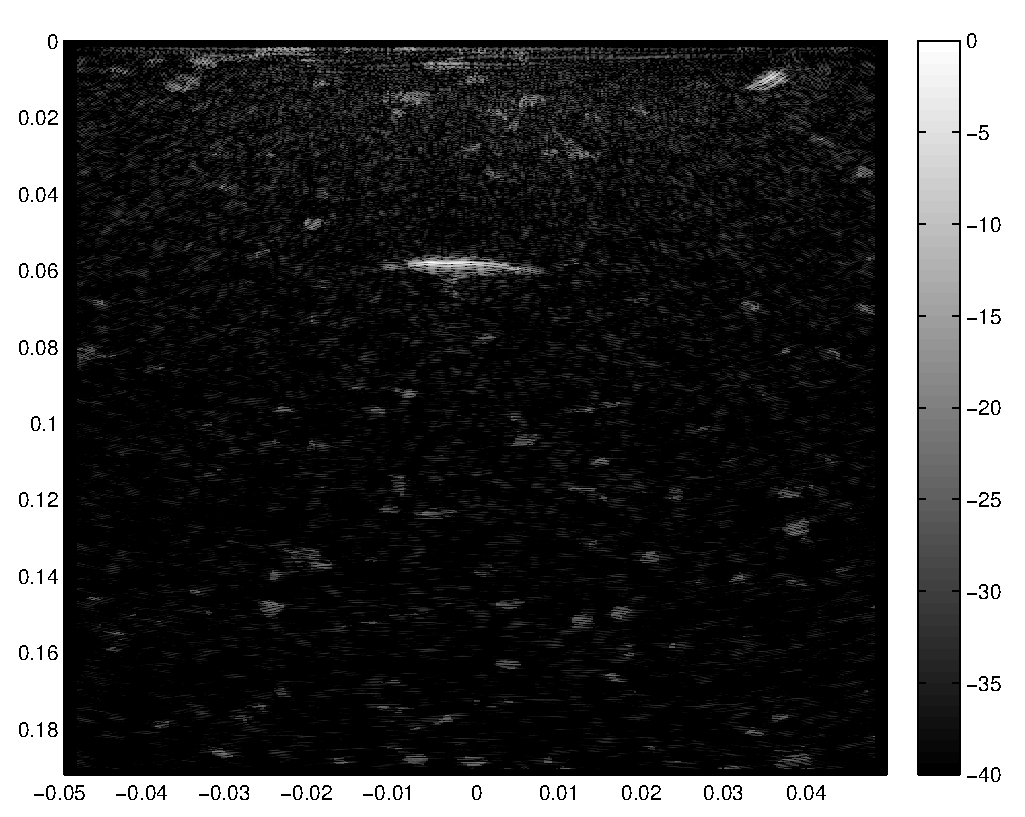
\includegraphics[width=100mm]{SAC_Common.eps}
		\caption{Common Midpoint Apodisation Result}
		\label{fig:apod_com_result}
\end{figure}

\begin{figure}[p]
\centering
		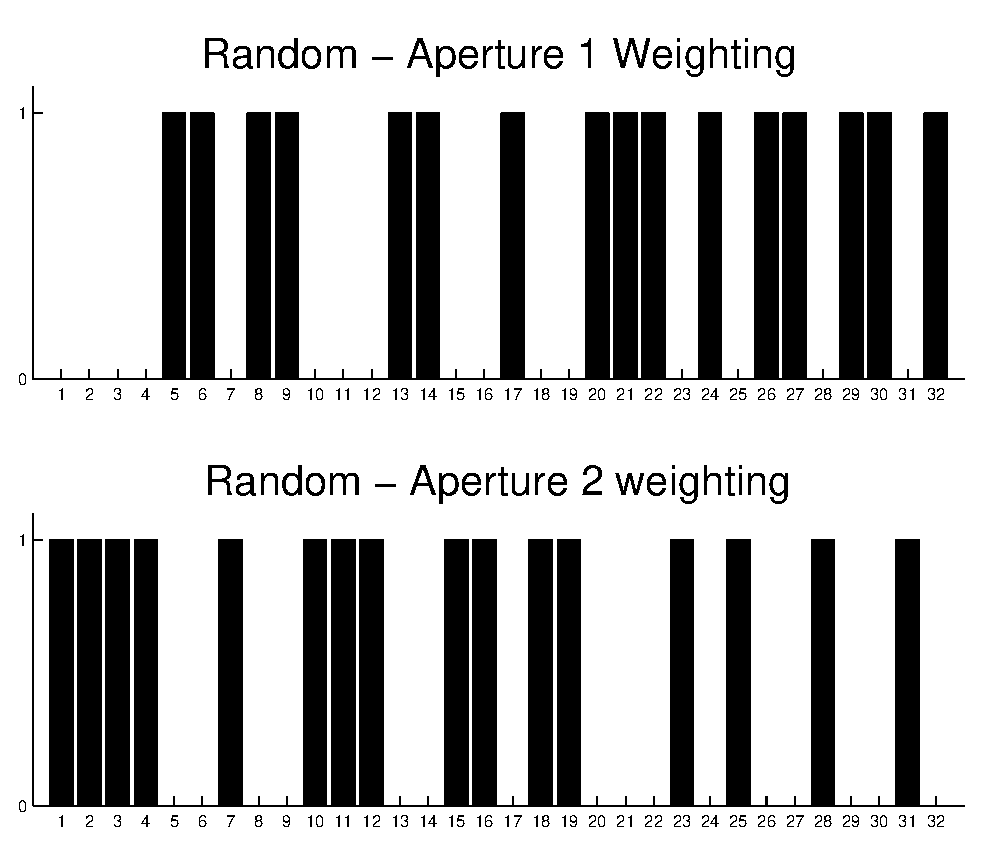
\includegraphics[width=100mm]{Random.eps}
		\caption{Random Apodisation}
		\label{fig:apod_ran}

		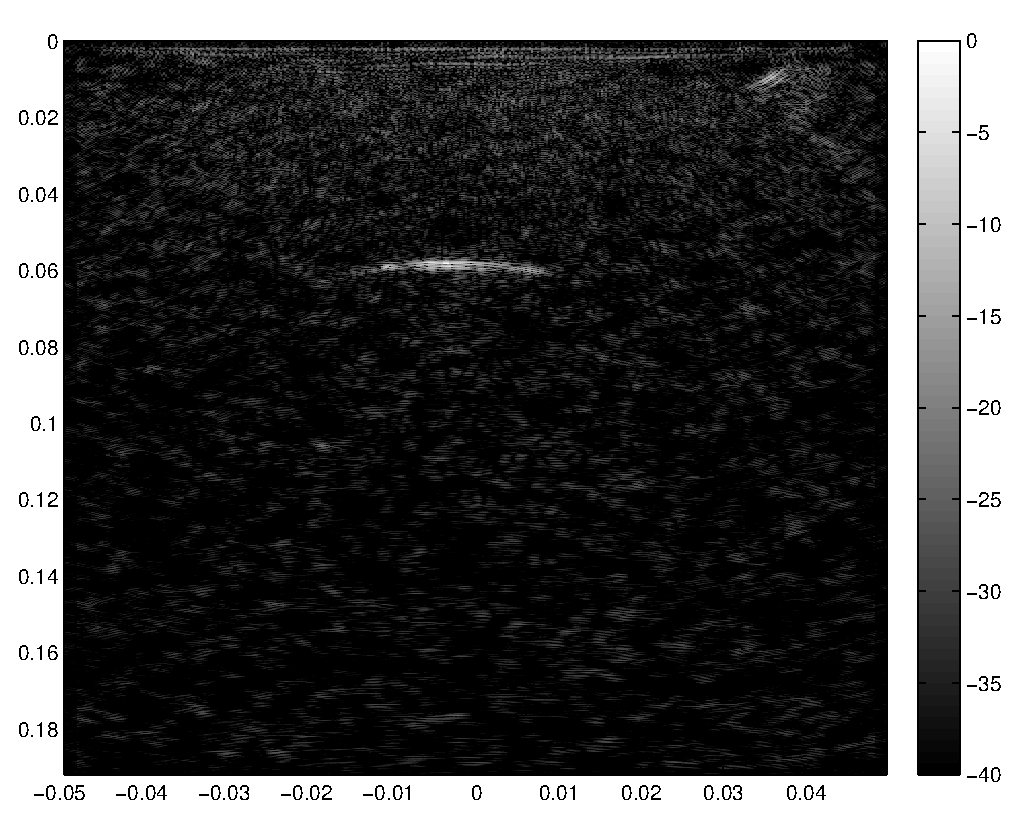
\includegraphics[width=100mm]{SAC_Random.eps}
		\caption{Random Apodisation Result}
		\label{fig:apod_ran_result}
\end{figure}
\clearpage
\subsection{Evaluation of Apodisation Methods}
The results from the apodisation methods discussed in the Section \ref{sec:sasaci_apodization} were evaluated to quantise their effectiveness. The signal-to-noise ratio (SNR) for each image was measured and tabulated (shown Table \ref{table:apod_methods}) so that the best of the image weightings could be identified. Using the known position for both side-drilled holes in the test block, the area where the reflection from the holes is above -6dB in the TFM image is considered signal. Everything else is considered noise. This method of differentiating signal and noise was chosen so that the poor focus on the 60mm side drilled hole would not be detrimental to the SNR in either the TFM or SASACI images. Instead, the SNR will be representative of the mean amplitude of the speckle noise in the images. A look-up matrix was generated for the current dataset so that signal and noise can quickly be calculated. This matrix is shown in Figure~\ref{fig:snr_result}, where the black areas are considered signal and the white areas considered noise.

\begin{figure}[htb]
\centering
		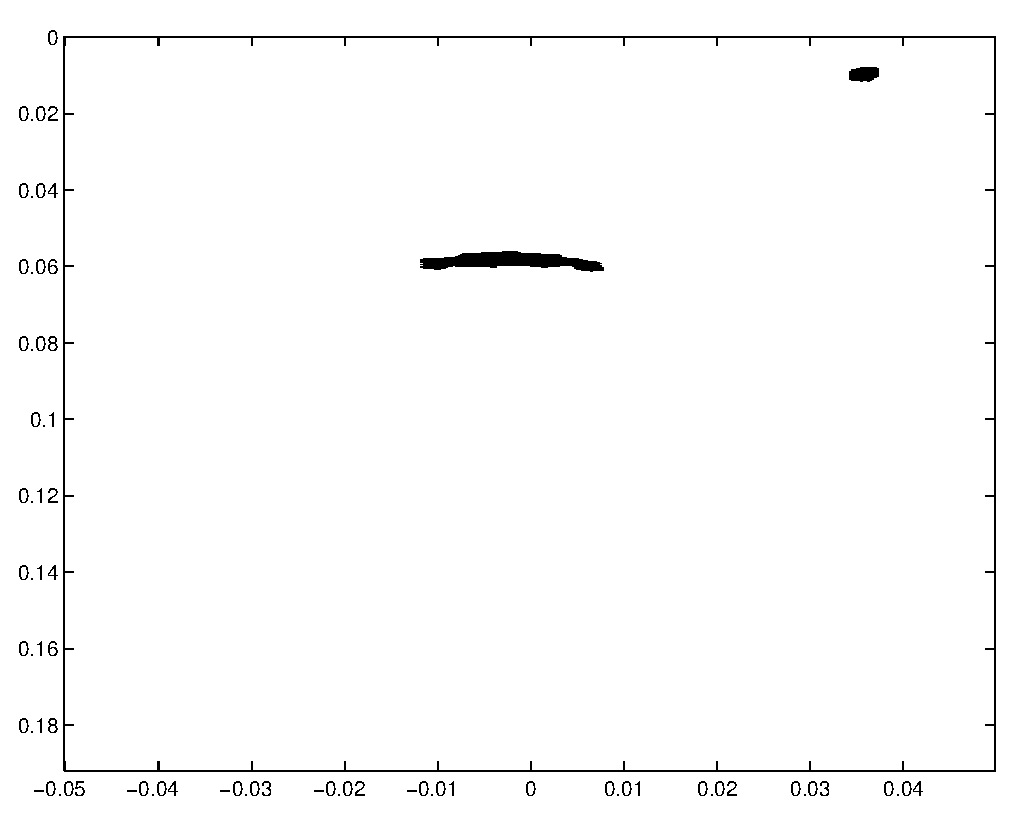
\includegraphics[width=100mm]{noise.eps}
		\caption{Locations of Signal and Noise}
		\label{fig:snr_result}
\end{figure}

	
In Table~\ref{table:apod_methods} it can be seen that the alternating apodisation technique is the best performing in this test scenario. It outperforms TFM by approximately 12dB. The random apodisation method is also effective, but due to the nature of the randomly generated apodisation weights the results differ each time that the algorithm runs. A number of averages could be taken to minimise the random component of these results, but this has not been investigated. Section \ref{sec:future_sasaci} discusses this in more detail.

\begin{table}[ht!]
\begin{center}
	\begin{tabular}{| c | c |}
	\hline 
	\textbf{Method} & \textbf{SNR} \\ \hline \hline 
	TFM	& 27.58dB \\ \hline
	Alternating & 39.55dB \\ \hline
	Common & 38.78dB \\ \hline
	Hamming & 31.80dB \\ \hline
	Hann & 34.03dB \\ \hline
	Random & 38.68dB \\ \hline
	\end{tabular}
	\caption{Comparison of Apodisation Methods}
	\label{table:apod_methods}
	\end{center}
	\end{table}
	
The alternating apodisation method was further investigated by altering the aperture widths. Alternating apertures with aperture widths of 1, 2, 4, 8, and 16 were created and images generated. The aperture shapes and resulting images can be seen in Figures \ref{fig:apod2} to~\ref{fig:apod16_result}. The resulting SNRs from these methods are shown in Table~\ref{table:alter_methods}. From this table, it can be observed that there appears to be an optimal aperture width, with SNR becoming poorer either side of the optimal value. In this case, the optimal aperture width was found to be 4 elements wide.
\begin{figure}[htbp]
\centering
		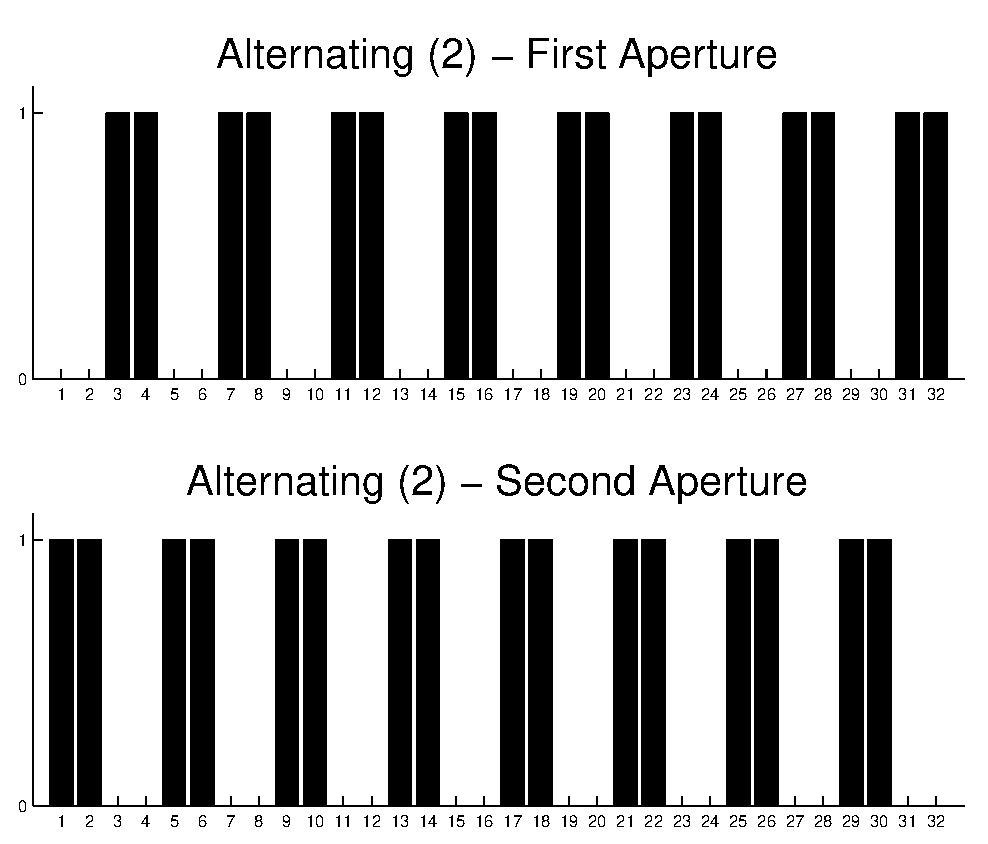
\includegraphics[width=100mm]{Alternating2.eps}
		\caption{Alternating Apodisation with 2x Aperture Width}
		\label{fig:apod2}

		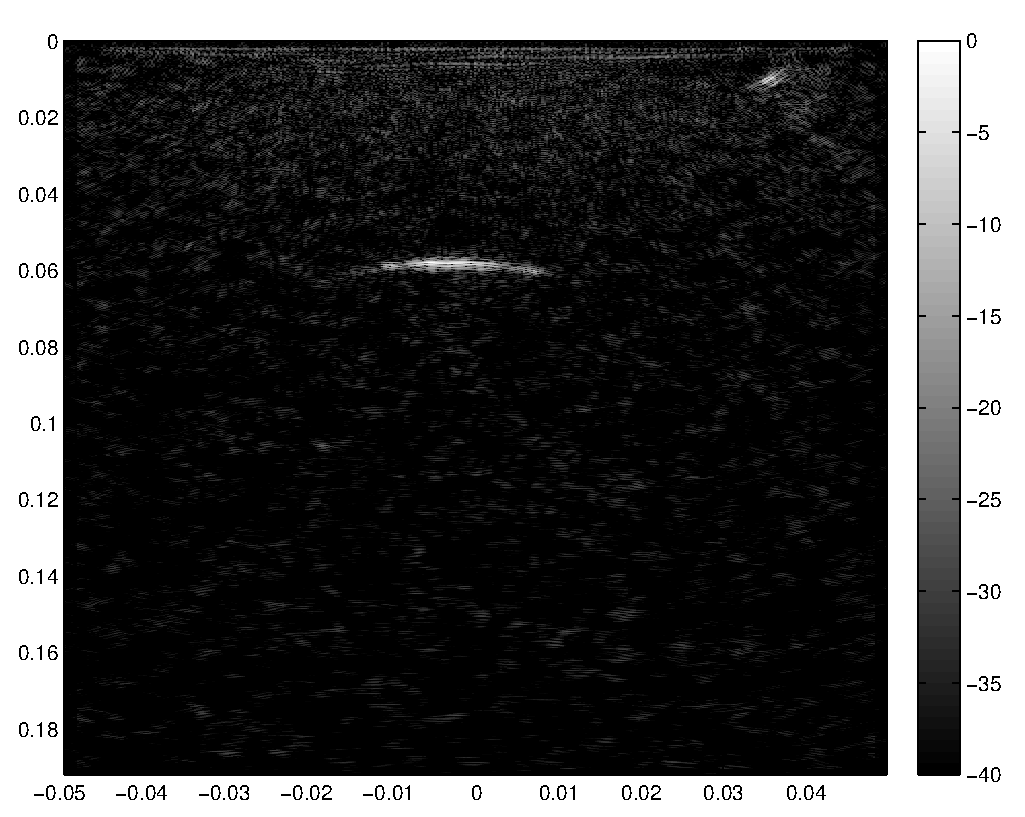
\includegraphics[width=100mm]{02_SAC.eps}
		\caption{Alternating Apodisation with 2x Aperture Width Result}
		\label{fig:apod2_result}
\end{figure}

\begin{figure}[htbp]
\centering
		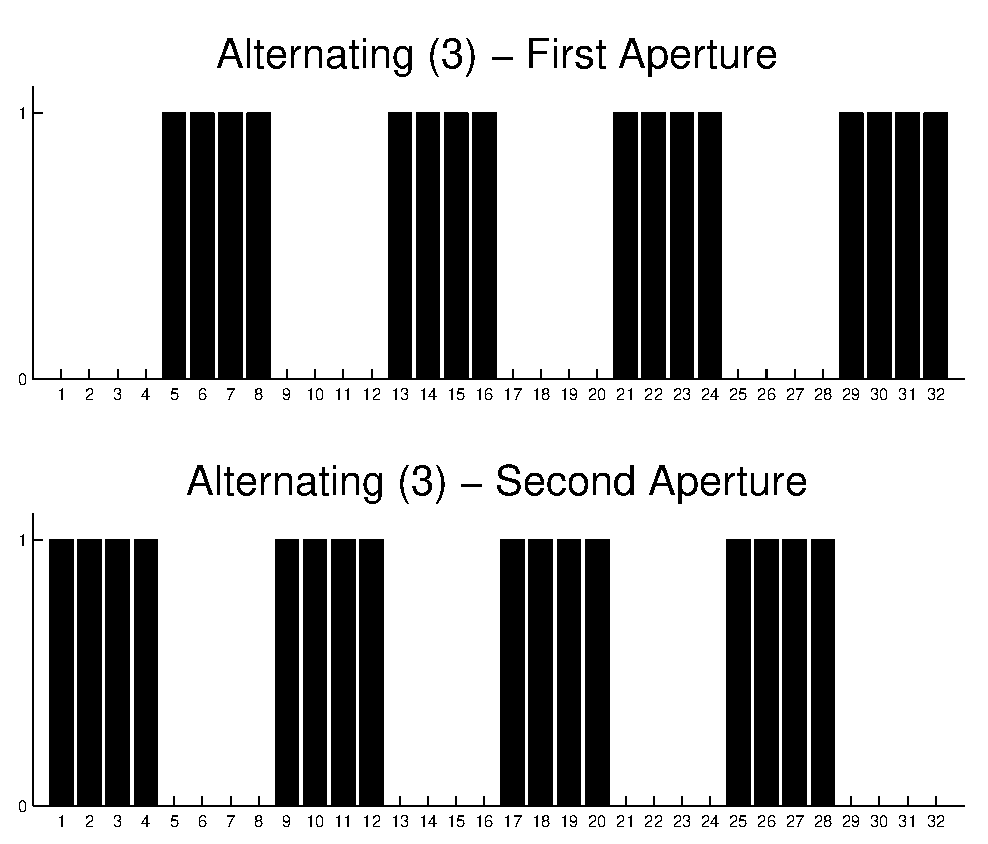
\includegraphics[width=100mm]{Alternating3.eps}
		\caption{Alternating Apodisation with 4x Aperture Width}
		\label{fig:apod4}

		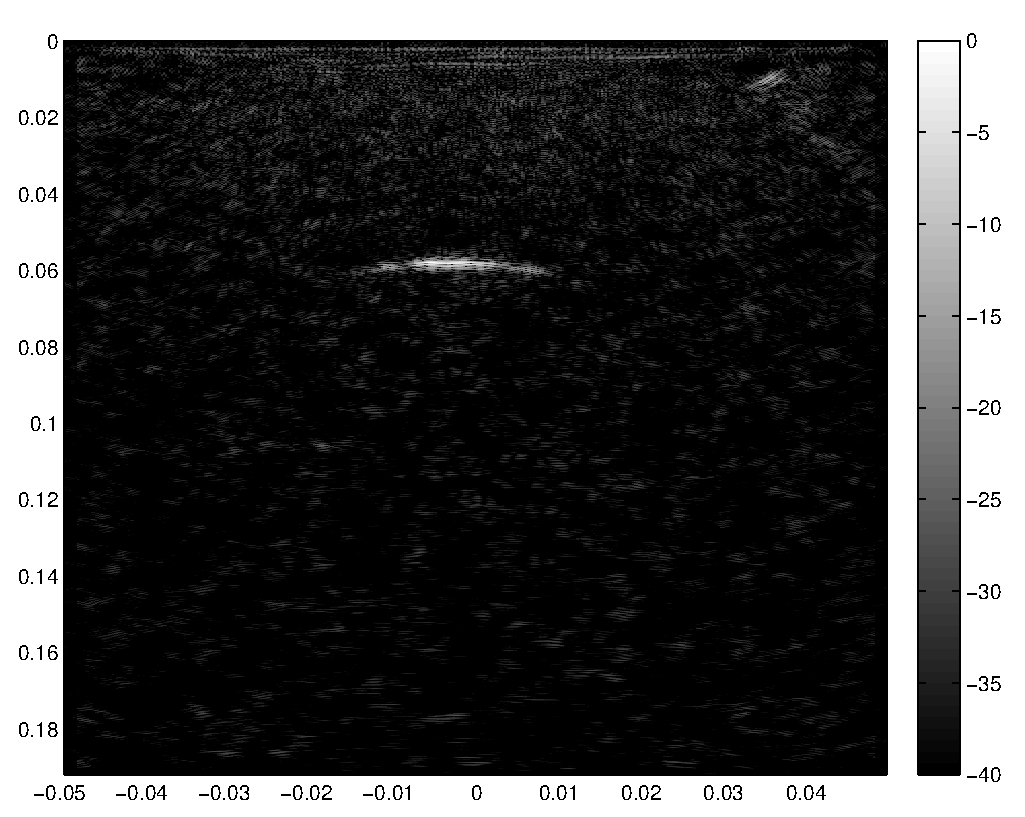
\includegraphics[width=100mm]{04_SAC.eps}
		\caption{Alternating Apodisation with 4x Aperture Width Result}
		\label{fig:apod4_result}
\end{figure}

\begin{figure}[htbp]
\centering
		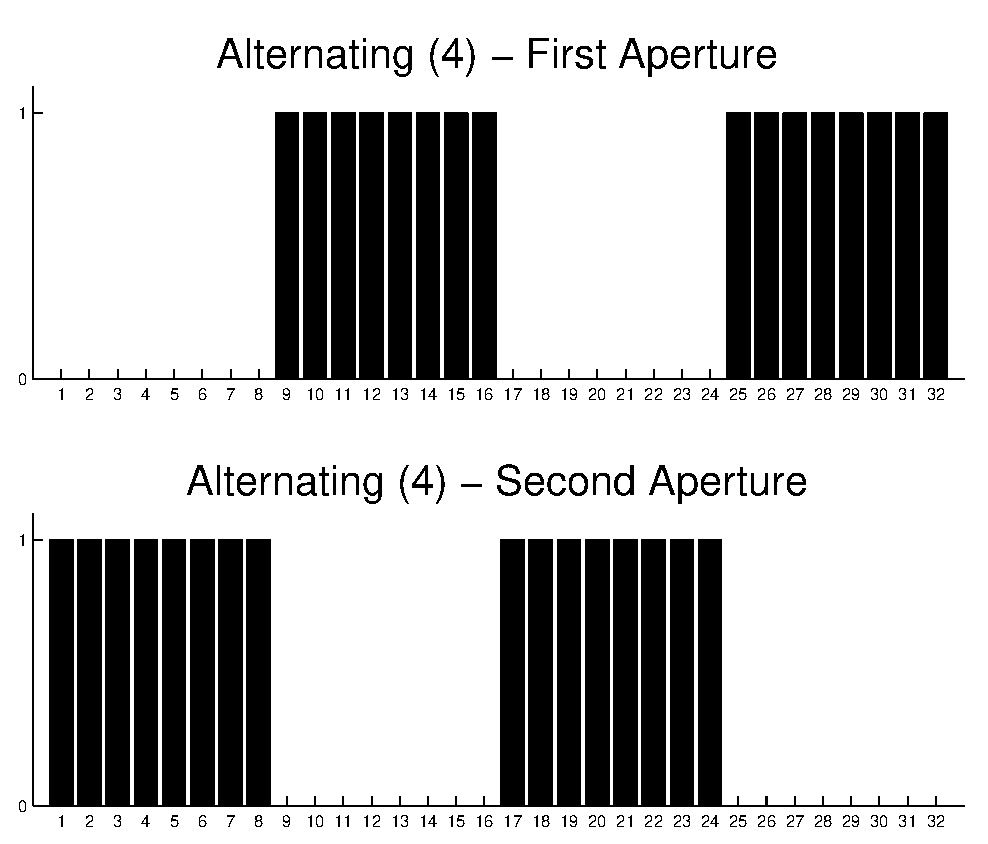
\includegraphics[width=100mm]{Alternating4.eps}
		\caption{Alternating Apodisation with 8x Aperture Width}
		\label{fig:apod8}

		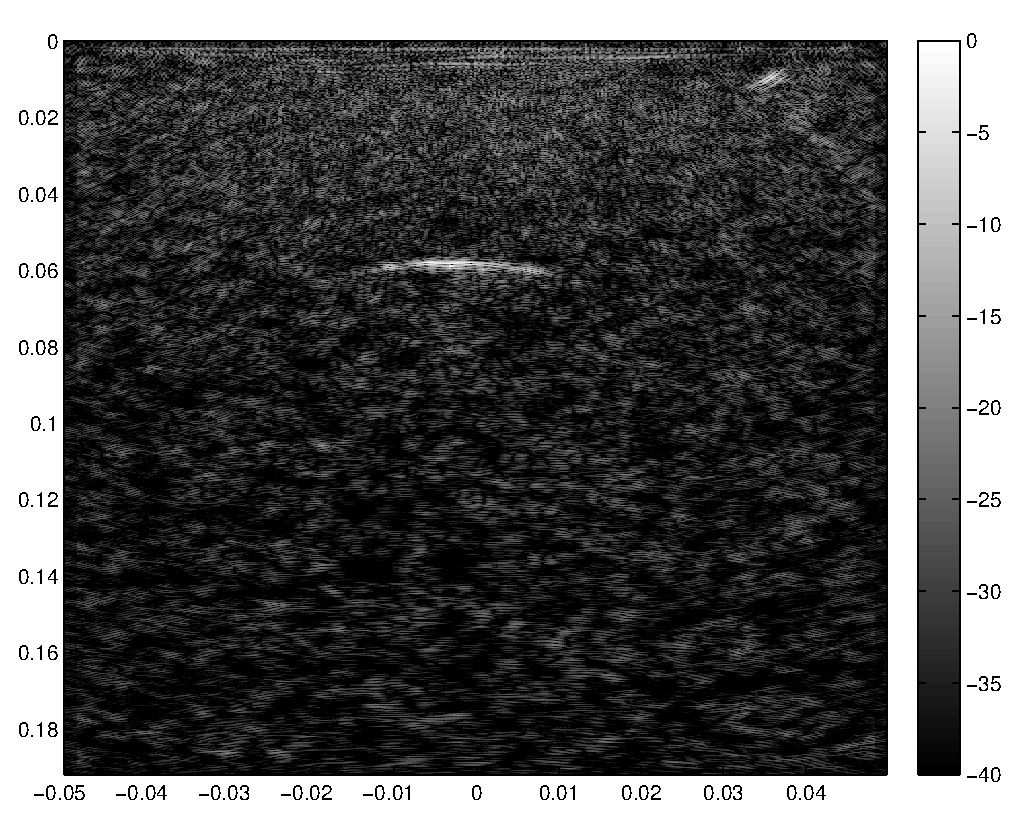
\includegraphics[width=100mm]{08_SAC.eps}
		\caption{Alternating Apodisation with 8x Aperture Width Result}
		\label{fig:apod8_result}
\end{figure}

\begin{figure}[htbp]
\centering
		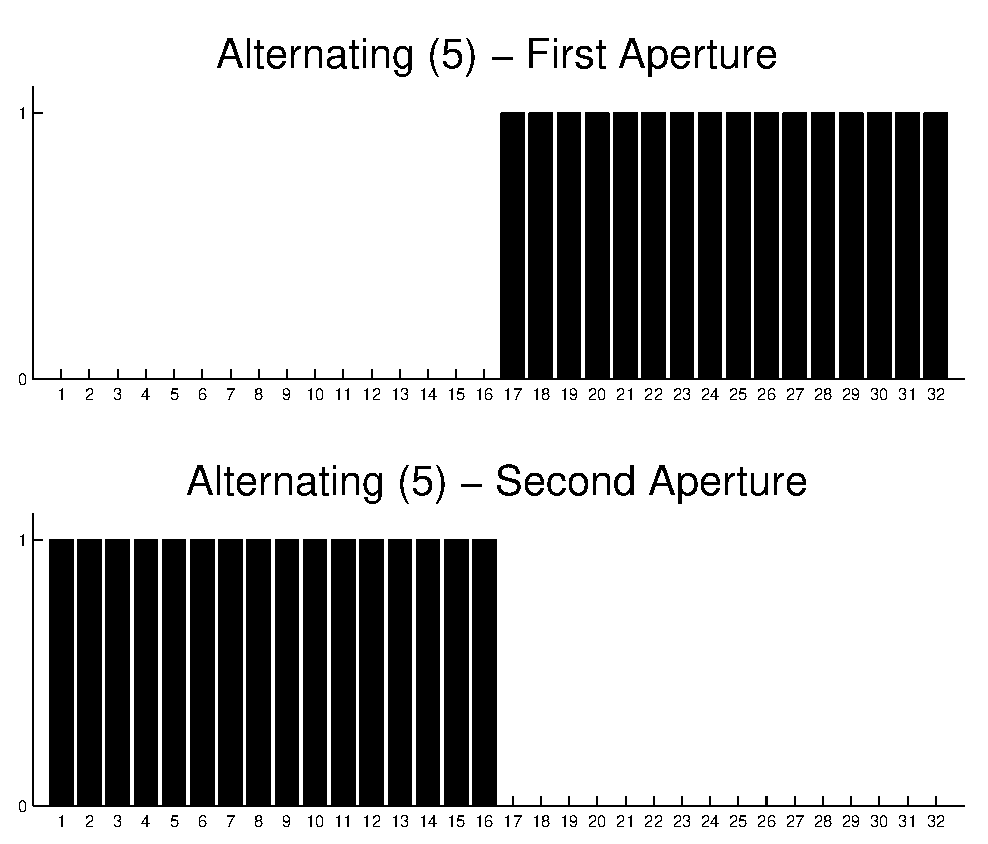
\includegraphics[width=100mm]{Alternating5.eps}
		\caption{Alternating Apodisation with 16x Aperture Width}
		\label{fig:apod16}


		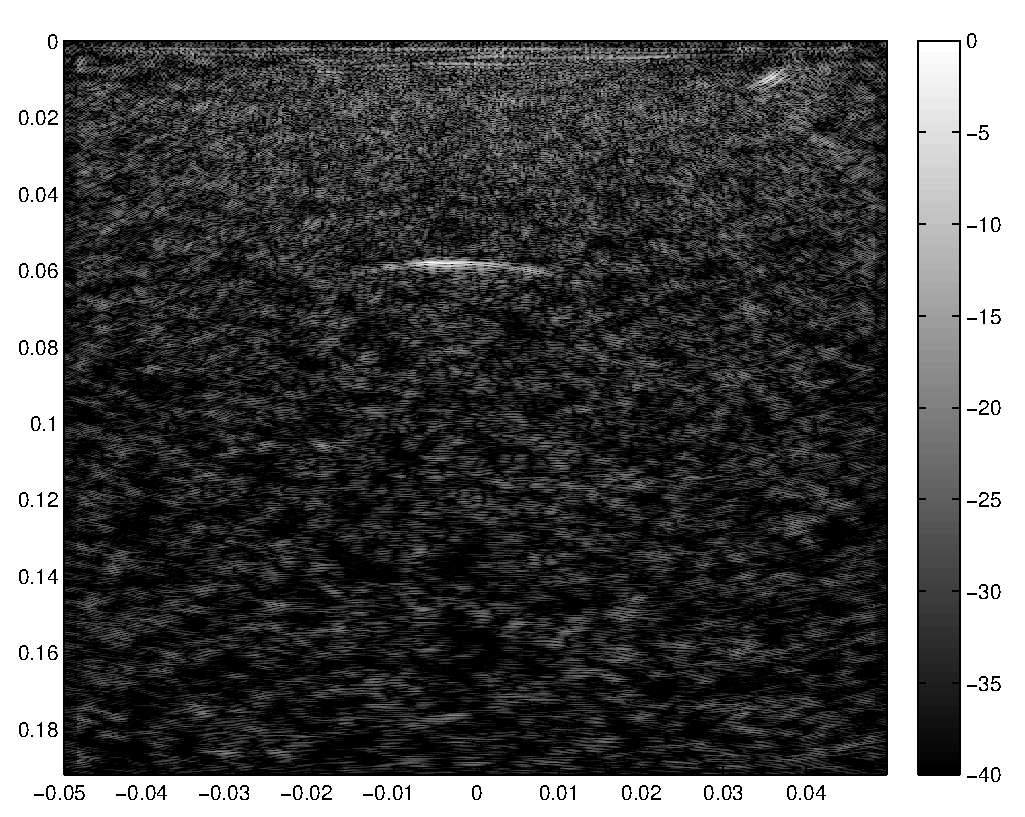
\includegraphics[width=100mm]{16_SAC.eps}
		\caption{Alternating Apodisation with 16x Aperture Width Result}
		\label{fig:apod16_result}
\end{figure}

\begin{table}[h!]
\begin{center}
	\begin{tabular}{| c | c |}
 	\hline 
	\textbf{Aperture Width (elements)} & \textbf{SNR} \\ \hline \hline 
	1	& 39.55dB \\ \hline
	2 & 40.29dB \\ \hline
	4 & 40.59dB \\ \hline
	8 & 32.30dB \\ \hline
	16 & 31.30dB \\ \hline
	\end{tabular}
	\caption{Comparison of Alternating Apodisation Aperture Widths}
	\label{table:alter_methods}
	\end{center}
	\end{table}
\clearpage
\section{Discussion}
A new signal processing technique for ultrasonic NDE has been proposed and experimental results demonstrated on a range of industrially relevant samples.

The SASACI approach involves creating two images of the same region. In this chapter, an investigation into improving imaging using sub-apertures from a single FMC dataset. It is anticipated that there are other ways to improve imaging using this methodology, using a set of arrays with differing centre frequencies, for example.

It was found the optimal way to weight the sub-TFM images is with an alternating scheme with a 4 element wide aperture. An maximum SNR improvement of 13dB has been achieved compared to a standard TFM image. Visually, defects appear clearer in SASACI images in a number of test cases, when compared to a bandpass-filtered TFM image. It can be concluded that this signal processing method is both novel and effective within the field of non-destructive evaluation of difficult materials.



% ------------------------------------------------------------------------


%%% Local Variables: 
%%% mode: latex
%%% TeX-master: "../thesis"
%%% End: 
